%!TEX root = ../main.tex
\chapter{Energy Scale Calibration of the AHCAL}
\label{chap:ECalibAHCAL}

The AHCAL was installed at the SPS CERN facilities in July 2015 in order to provide energy and time measurements of electromagnetic and hadronic showers. The data recorded in each cell of the calorimeter is measured in ADC counts. Channel-to-channel differences in light yield and SiPM gain make difficult channel-to-channel comparisons using this scale. Therefore, all channels have to be scaled to a common physical energy unit that suppresses these differences. For the AHCAL, the Minimum Ionizing Particle or MIP unit is chosen. This unit relates to the cell energy in a well understood physical process.

The conversion requires a calibration of each cell of the calorimeter which is by itself a challenge due to the high number of readout channels. For this thesis, 3744 channels have to be calibrated. Due to the AHCAL boards (see section \ref{sec:TBsetup}) equipped with various types of SiPMs, the procedure needs to be automatic and robust to extract the calibration constant for each channel.

In this chapter, the first section will described the procedure for the AHCAL energy scale calibration. The second section will present the results of the energy scale calibration as well as a comparison with simulation to validate the calibration. In this thesis, only the calibration of the energy scale of the detector was performed. A dedicated analysis of the performance of the detector is being performed in parallel \cite{AmbraEnergy, AmbraTokyo}.

\section{Energy Calibration of the AHCAL}
\label{sec:EnergyCalibration}

The energy deposited by a charged particle in a single AHCAL cell follows approximatively a Landau distribution (see section \ref{sec:PartInter}) but due to the electronic noise, the resulting response is convoluted with a Gaussian distribution. The maximum of the Laudau-Gaussian convolution density function is defined as the MIP constant ($M_{i}$) for the i-th channel. The conversion to the MIP energy scale for a AHCAL cell is expressed as:
\begin{equation}
	E_i = \frac{(A_i - P_i) \times IC_i }{\frac{M_{i}}{ICP_i}}
\end{equation}

where $E_i$ is the calibrated amplitude in MIP, $A_i$ is the measured amplitude in ADC, $P_i$ is the pedestal in ADC, $ICP_i$ is the intercalibration factor between calibration and physics mode specific to the layers 4 and 5 (see section \ref{sec:AdjustGain}), $IC_i$ is the intercalibration factor between High/Low gain (see section \ref{sec:SPIROC2B}) and $M_{i}$ is the MIP constant of the i-th channel in $\frac{ADC}{MIP}$. SiPMs have a finite number of pixel thus their signal saturates for a high number of scintillation photons. One can correct the hit energy for the saturation effect with the following formula:
\begin{equation}
	E_i = \frac{f^{i}_{unsat}( (A_i - P_i) \times \frac{IC_i \times ICP_i}{G_i} )}{LY_{i}}
\end{equation}

where $f^{i}_{unsat}$ is the inverse SiPM saturation function (see section \ref{sec:SiPM}) and $LY_{i} = \frac{M_{i}}{G_i}$ is the light yield of the i-th channel.

\subsection{Pedestal extraction}

The baseline or pedestal needs to be subtracted to the signal to obtain the MIP calibration constant for each channel. The pedestal value for each channel is extracted from the data taking muon runs. In order to be consistent, the pedestal value is extracted in the same running mode as the recorded data, i.e. in auto-trigger (AT) \cite{Hermberg:2015gaa, SarahMaster}.

The pedestal distribution of a typical AHCAL channel is shown in figure \ref{fig:PedExtraction}. A histogram is filled with the ADC value per readout cycle. This is only done for channels where the HitBit is not set (see section \ref{sec:SPIROC2B}). The extraction of the pedestal value is performed in an iterative way due to a high energy tail that is not yet understood and could come from an inefficiency in the trigger threshold.

\begin{figure}[htbp!]
	\centering
	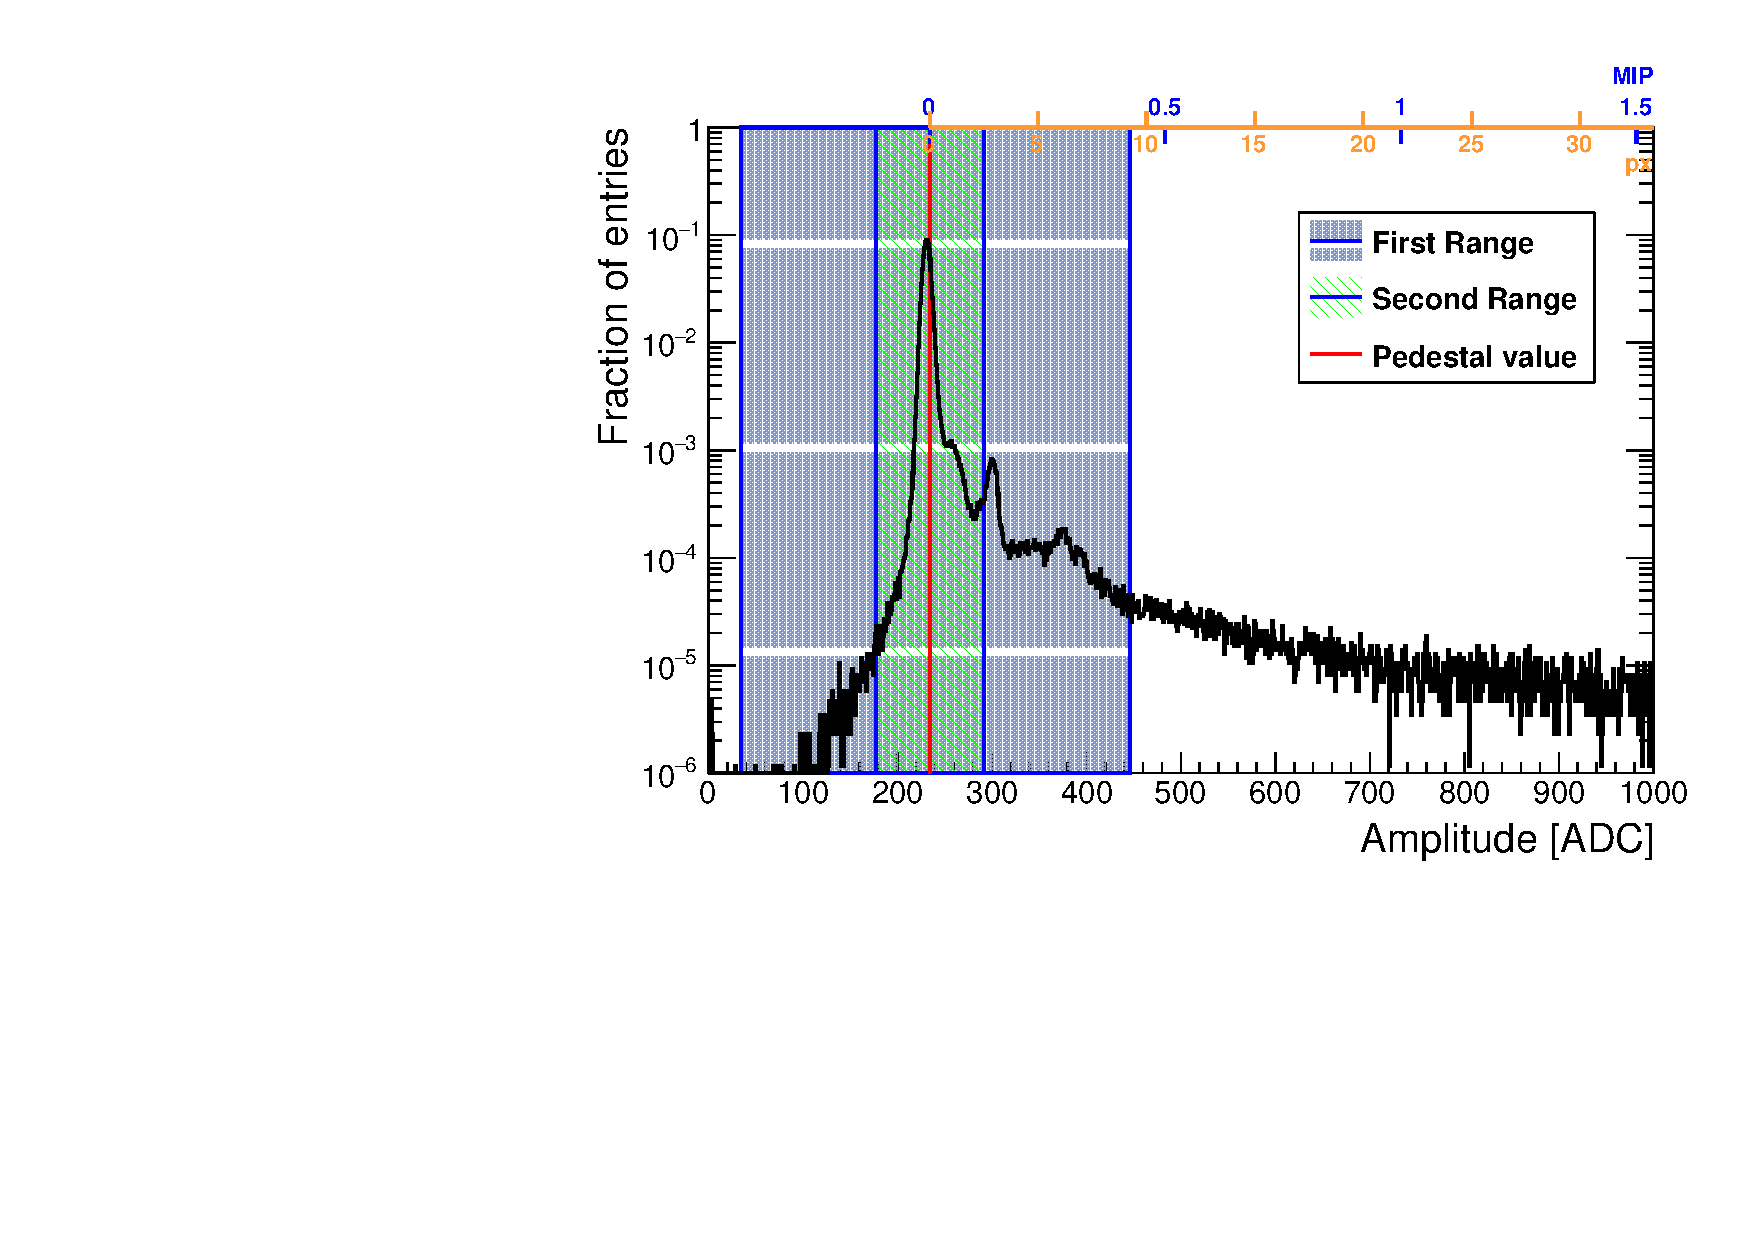
\includegraphics[width=0.6\linewidth]{../Thesis_Plots/EnergyCalib/Plots/PedestalExtractionExample.pdf}
	\caption{Typical pedestal distribution of a channel in auto-trigger mode. The different colored boxed represent the iterative procedure to extract the pedestal value marked with the red line. The upper x-axis shows the corresponding ADC value in terms of MIP and pixels.} \label{fig:PedExtraction}
\end{figure}

The SiPM noise contributes to the pedestal value as shown by the additional peaks next to the main peak in the figure \ref{fig:PedExtraction}. Considering a Poisson statistic, one to three pixels could be fired due to the dark noise and cross-talk. The range to determine the pedestal value then needs to be in the same order of magnitude. For this, the histogram x-axis range is reduced in the range of 3 RMS around the mean. It is done iteratively two times. Then the mean of the histogram is taken as the pedestal value. This is done for each channel and memory-cell.

However, the CALICE database structure, containing the main calibration constants, is designed to store the pedestal constant for each channel only (not memory-cell). Therefore, a mean over all memory cells is computed per channel and used in the data reconstruction. The difference between the mean pedestal and the memory cell wise pedestal is shown in figure \ref{fig:CompMeanMem}. The RMS of the distribution is around 21 ADC which would correspond to an uncertainty of about 4\% on the MIP constant, assuming a typical MIP calibration value of 500 ADC. This error is dominating in the MIP constant uncertainty.

\begin{figure}[htbp!]
	\centering
	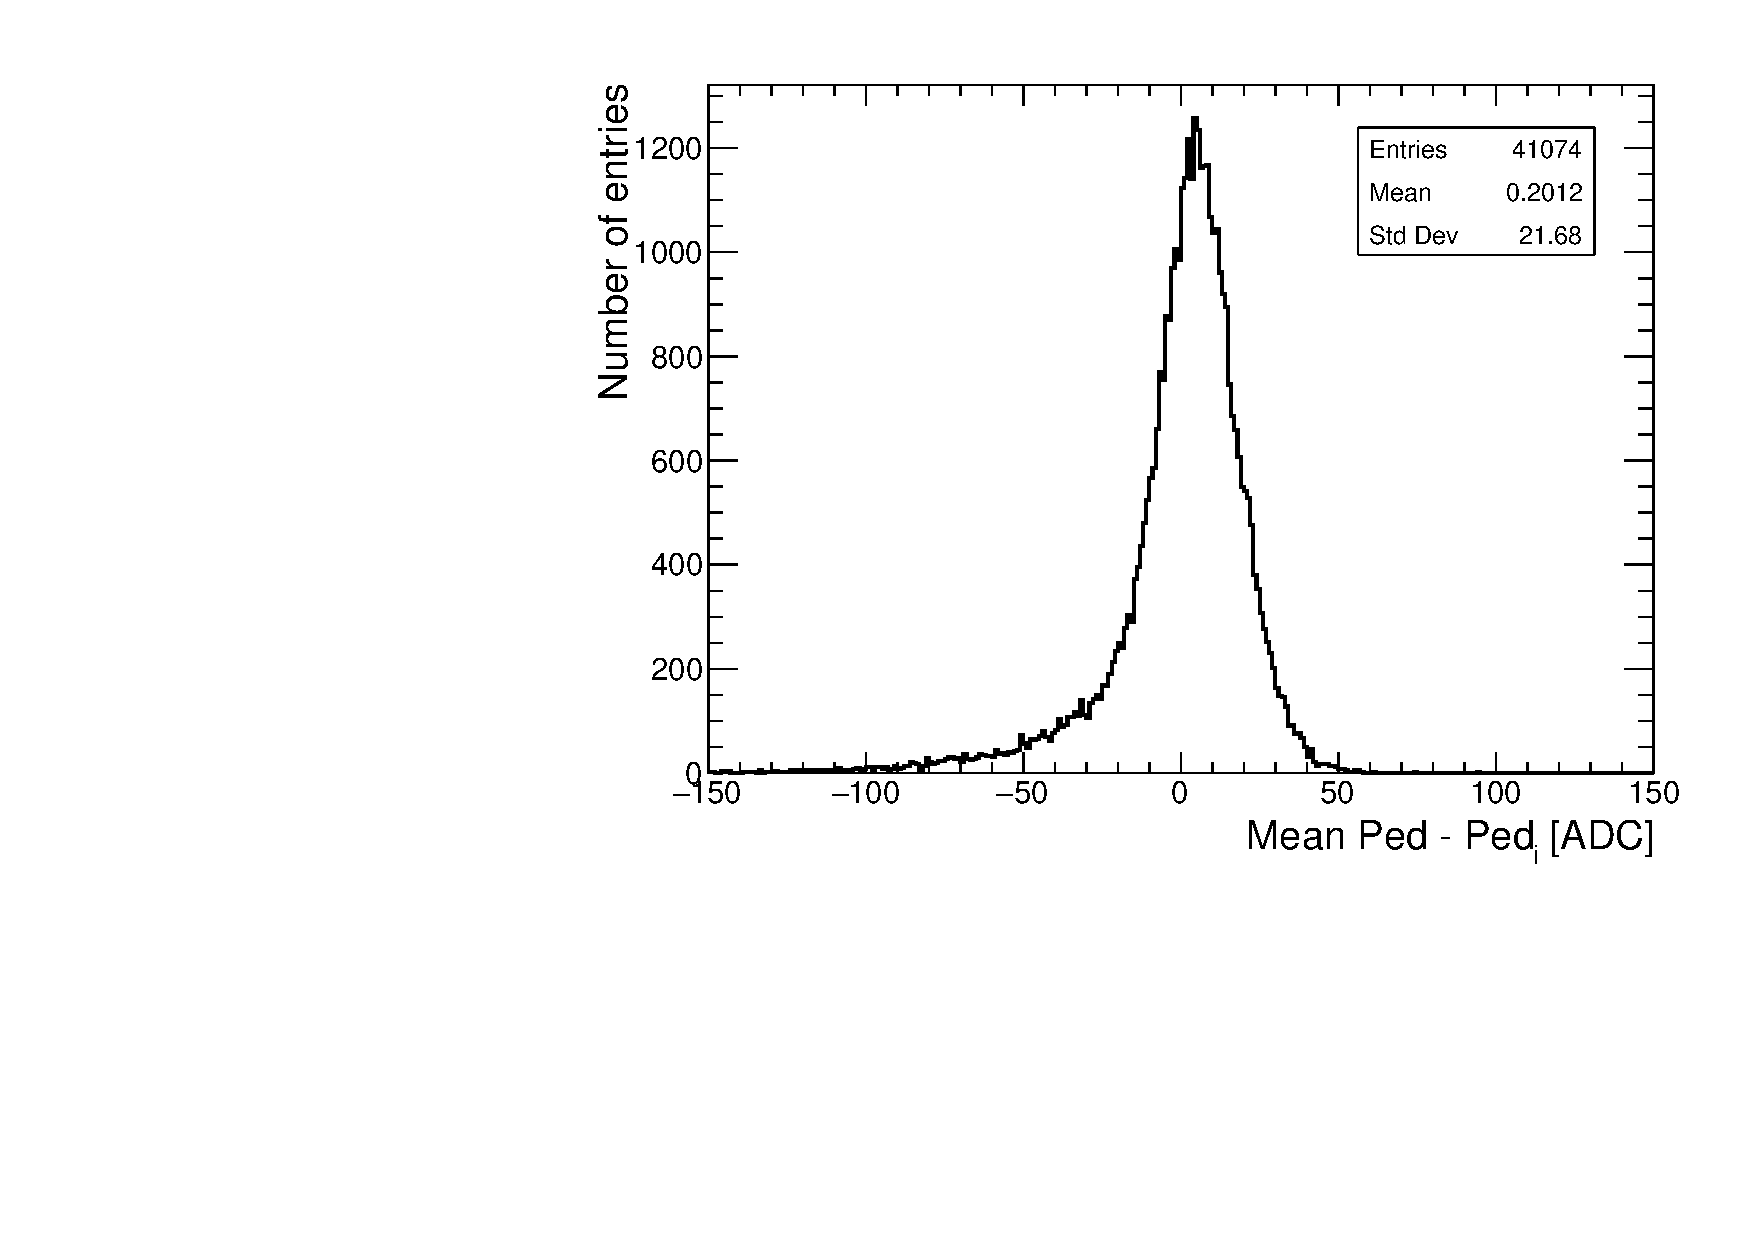
\includegraphics[width=0.6\linewidth]{../Thesis_Plots/EnergyCalib/Plots/ComparisonMeanPedtoMemorycell.pdf}
	\caption{Distribution of the difference between the mean pedestal to the memory-cell wise pedestal per channel.} \label{fig:CompMeanMem}
\end{figure}

\subsection{MIP extraction}
\label{sec:MIPExtraction}

After the pedestal calibration, the extraction of the MIP calibration constant for each channel can be performed. As the detector was equipped with various types of SiPM and boards designs, the extraction procedure needs to be automatic and robust. In order to reduce the amount of noise hits in the hit energy spectra of each cell that would lead to unstable fits and wrong MIP calibration constants, a MIP track selection has been performed (see section \ref{subsec:Muon_sel}).

The fitting procedure is very sensitive to the initial parameters of the fit and can be quite difficult with the variety of SiPM and tiles in the AHCAL. To ensure a good fit, an iterative fitting procedure is performed. A more precise and detailed description of the fitting procedure is explained in \cite{FabianThesis, SarahMaster}.

\begin{figure}[htbp!]
	\centering
	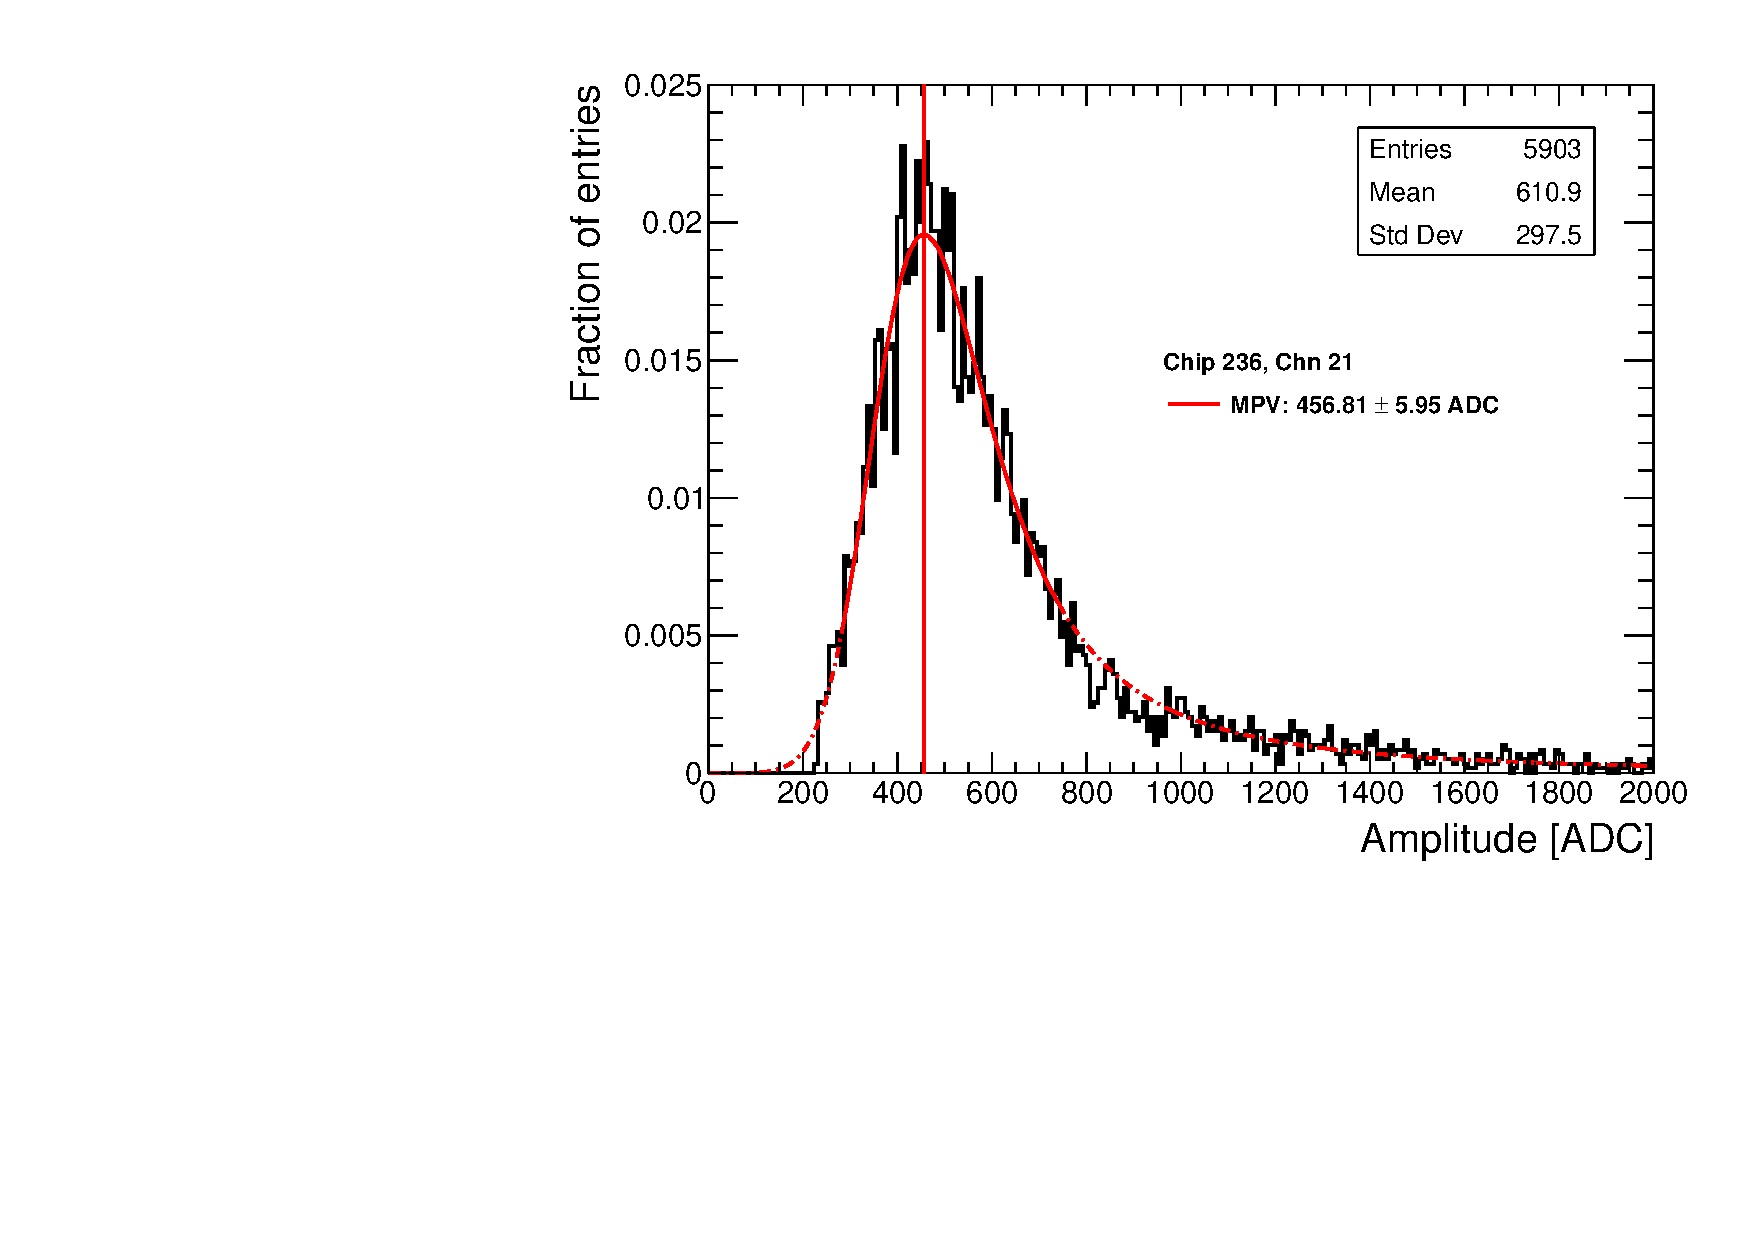
\includegraphics[width=0.6\linewidth]{../Thesis_Plots/EnergyCalib/Plots/ExampleMIP_Module3.pdf}
	\caption{Typical energy distribution in a single channel of the AHCAL with the data collected in July 2015 at CERN. The convoluted function is represented in red with the extracted MIP constant for this channel showed by the vertical red line.} \label{fig:MIPFit}
\end{figure}

Only channels with more than 1000 entries are considered to obtain a reliable fit. The parameters in the fit are: the area of the hit energy distribution, the width of the convoluted Gaussian, the most probable value (MPV) of the Landau distribution and the width of the Landau distribution. The spectrum of the hit energy is fitted with a Laudau-Gaussian convolution function for each channel and the maximum of this convoluted function is taken as the MIP constant. A typical example of a single channel fit can be seen in figure \ref{fig:MIPFit}. The fit result has been verified channel-by-channel for all the channels of the detector.

\section{Results of the energy scale calibration}

\subsection{MIP extraction results}

In the muon data recorded in July 2015, the MIP calibration constant of 72\% of the 3744 channels is determined. The rest 28\% of the channels does not provide enough or usable information to perform a fit, this includes the outer channels (outside of the inner $12 \times 12$ tiles) of the layers 11 to 14 that don't have enough statistics. In order to have a MIP calibration value for these outer channels, the results are combined with MIP calibration values obtained from previous testbeams performed in April and May 2015 at DESY with the layers 11 to 14.

Additionally, if a channel does not have a MIP calibration value, the mean of the MIP constant distribution of a chip or a layer is used. 85\% of the detector channels (3171 channels) have been calibrated, excluding dead and noisy channels (see appendix \ref{appendix:deadChn}).

The results of the extracted MIP values are shown in table \ref{table:MIPAHCAL} and are regrouped by SiPM types. The results are well compatible with previous work \cite{SarahMaster} although there is slight difference in the number of fitted channels that may come from the differences in the event selection and the extraction procedure.

\begin{table}[htb!]
	\centering
	\caption{Table containing the results of the extraction of the MIP calibration constants. The results are regrouped by SiPM type. <MIP> is the mean of the MIP calibration constant distribution per SiPM type. RMS is the standard deviation of MIP calibration constant distribution per SiPM type. Dead and noisy channels are rejected.}
	\label{table:MIPAHCAL}
	\begin{tabular}{@{} lccc @{}}
		\toprule
		Layer \# & <MIP> [ADC] & RMS [ADC] & $N_{fitted}$\\
		\midrule
		1-2 & 66.72 & 35.54 & 172\\
		3 & 501.71 & 50.4 & 142\\
		4-5 & 796.54 & 113.12 & 265\\
		6-10 & 250.99 & 62.72 & 414\\
		11-12 & 285.85 & 62.83 & 1069\\
		13-14 & 307.73 & 58.96 & 1109\\
		\bottomrule
	\end{tabular}
\end{table}

\subsection{Uncertainty of the calibration procedure}

It is necessary to evaluate the uncertainty of the calibration procedure. The figure \ref{fig:MIPError} shows the relative error $\frac{\Delta MIP_i}{MIP_i}$ for all the channels of the detector. The relative error on the MIP calibration value, for most of the channels, is in the expected range of 1\% to 3\% and it is compatible with previous results \cite{SarahMaster}. However, some higher values can be seen due to the layers 1 and 2 where difficulties were met due to a high noise and low SiPM gain.

\begin{figure}[htbp!]
	\centering
	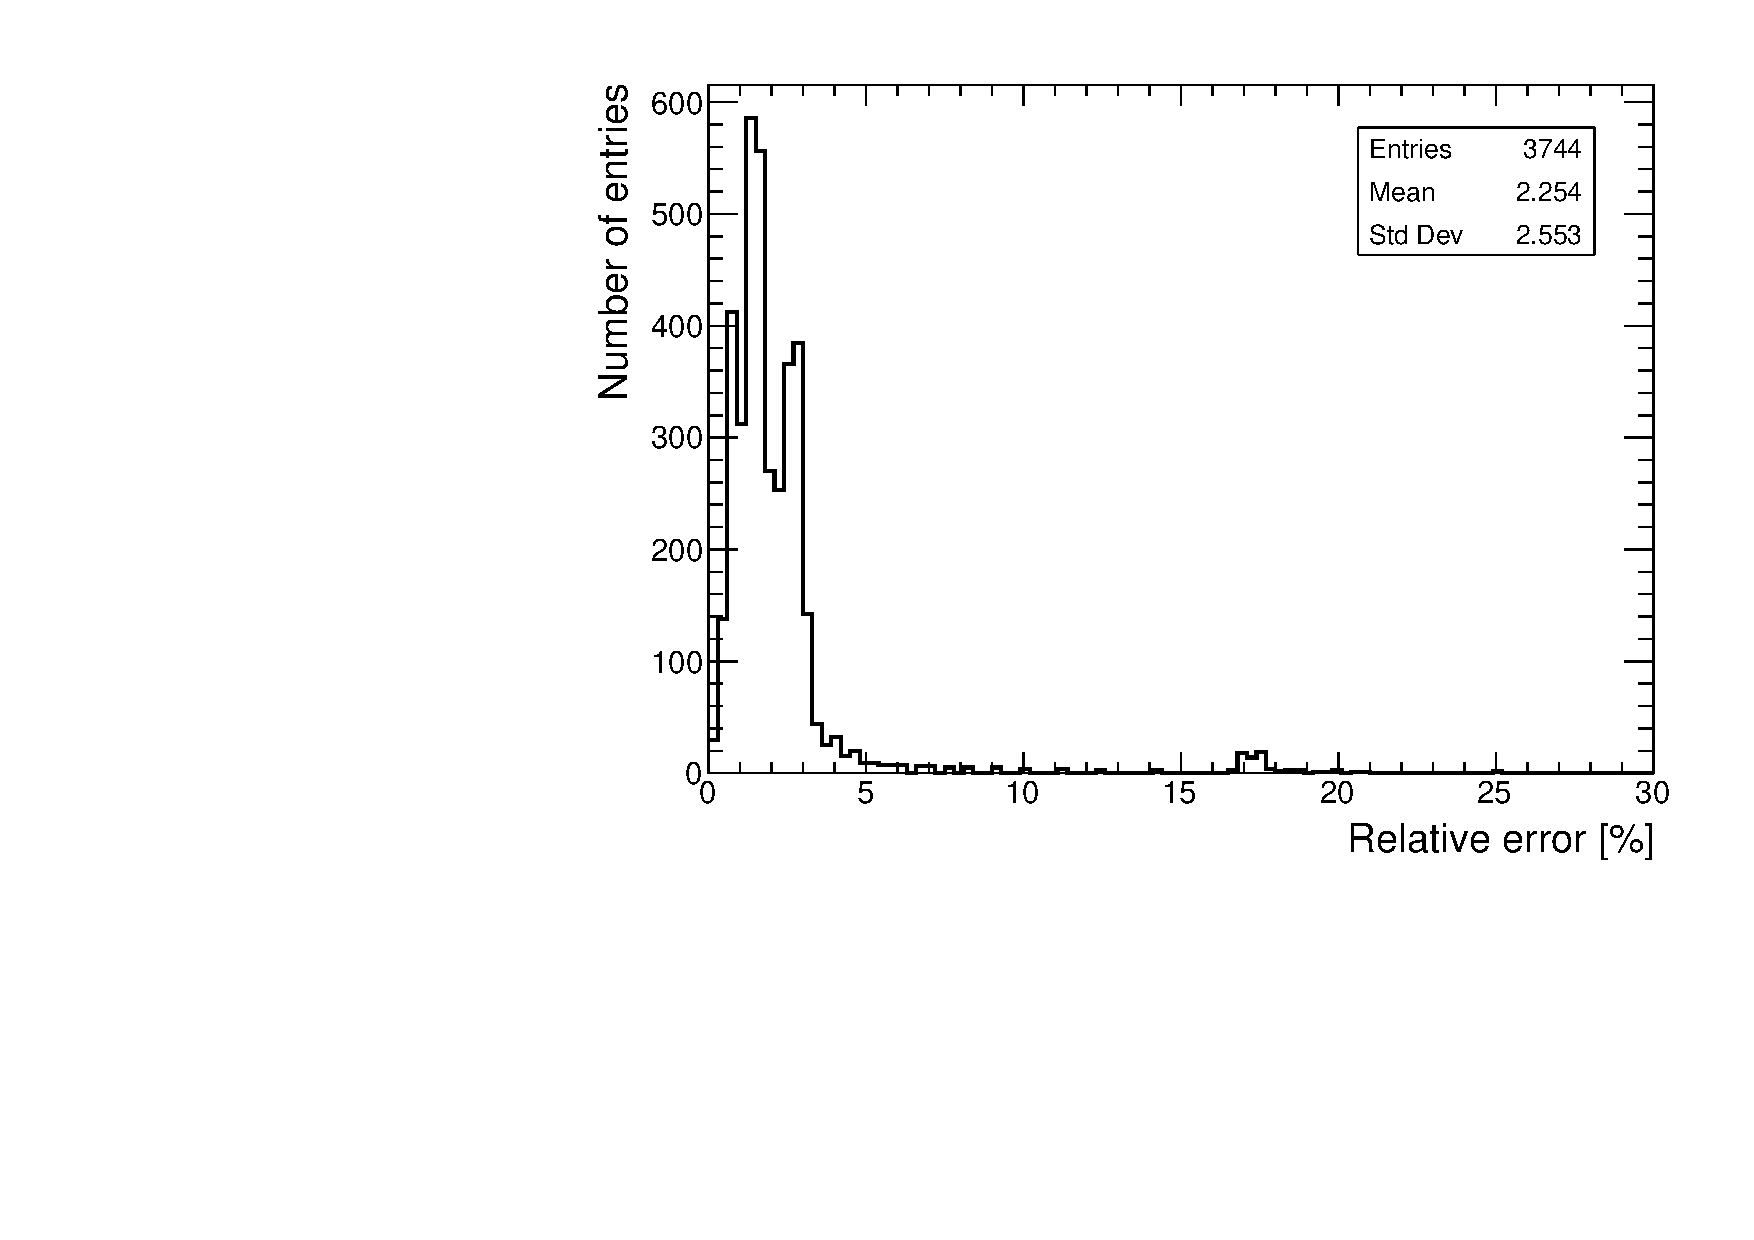
\includegraphics[width=0.6\linewidth]{../Thesis_Plots/EnergyCalib/Plots/RelativeErrorMIP_Combined.pdf}
	\caption{Relative error $\frac{\Delta MIP_i}{MIP_i}$ for the 3171 detector channels in the AHCAL.} \label{fig:MIPError}
\end{figure}

\subsection{Systematic on the MIP scale}

The MIP constant value is sensitive to temperature and temporal variations. A systematic error on the MIP energy scale can be derived by dividing the data muon sample into two sub-samples by even or odd run number. It will take into account the uncertainty on the MIP calibration but as well temperature and temporal variations. Each sub-sample is fitted using the same fitting procedure as described in section \ref{sec:MIPExtraction}. The results of the MIP fit for each sub-samples are shown in figure \ref{fig:MIPSyst}.

\begin{figure}[htbp!]
	\centering
	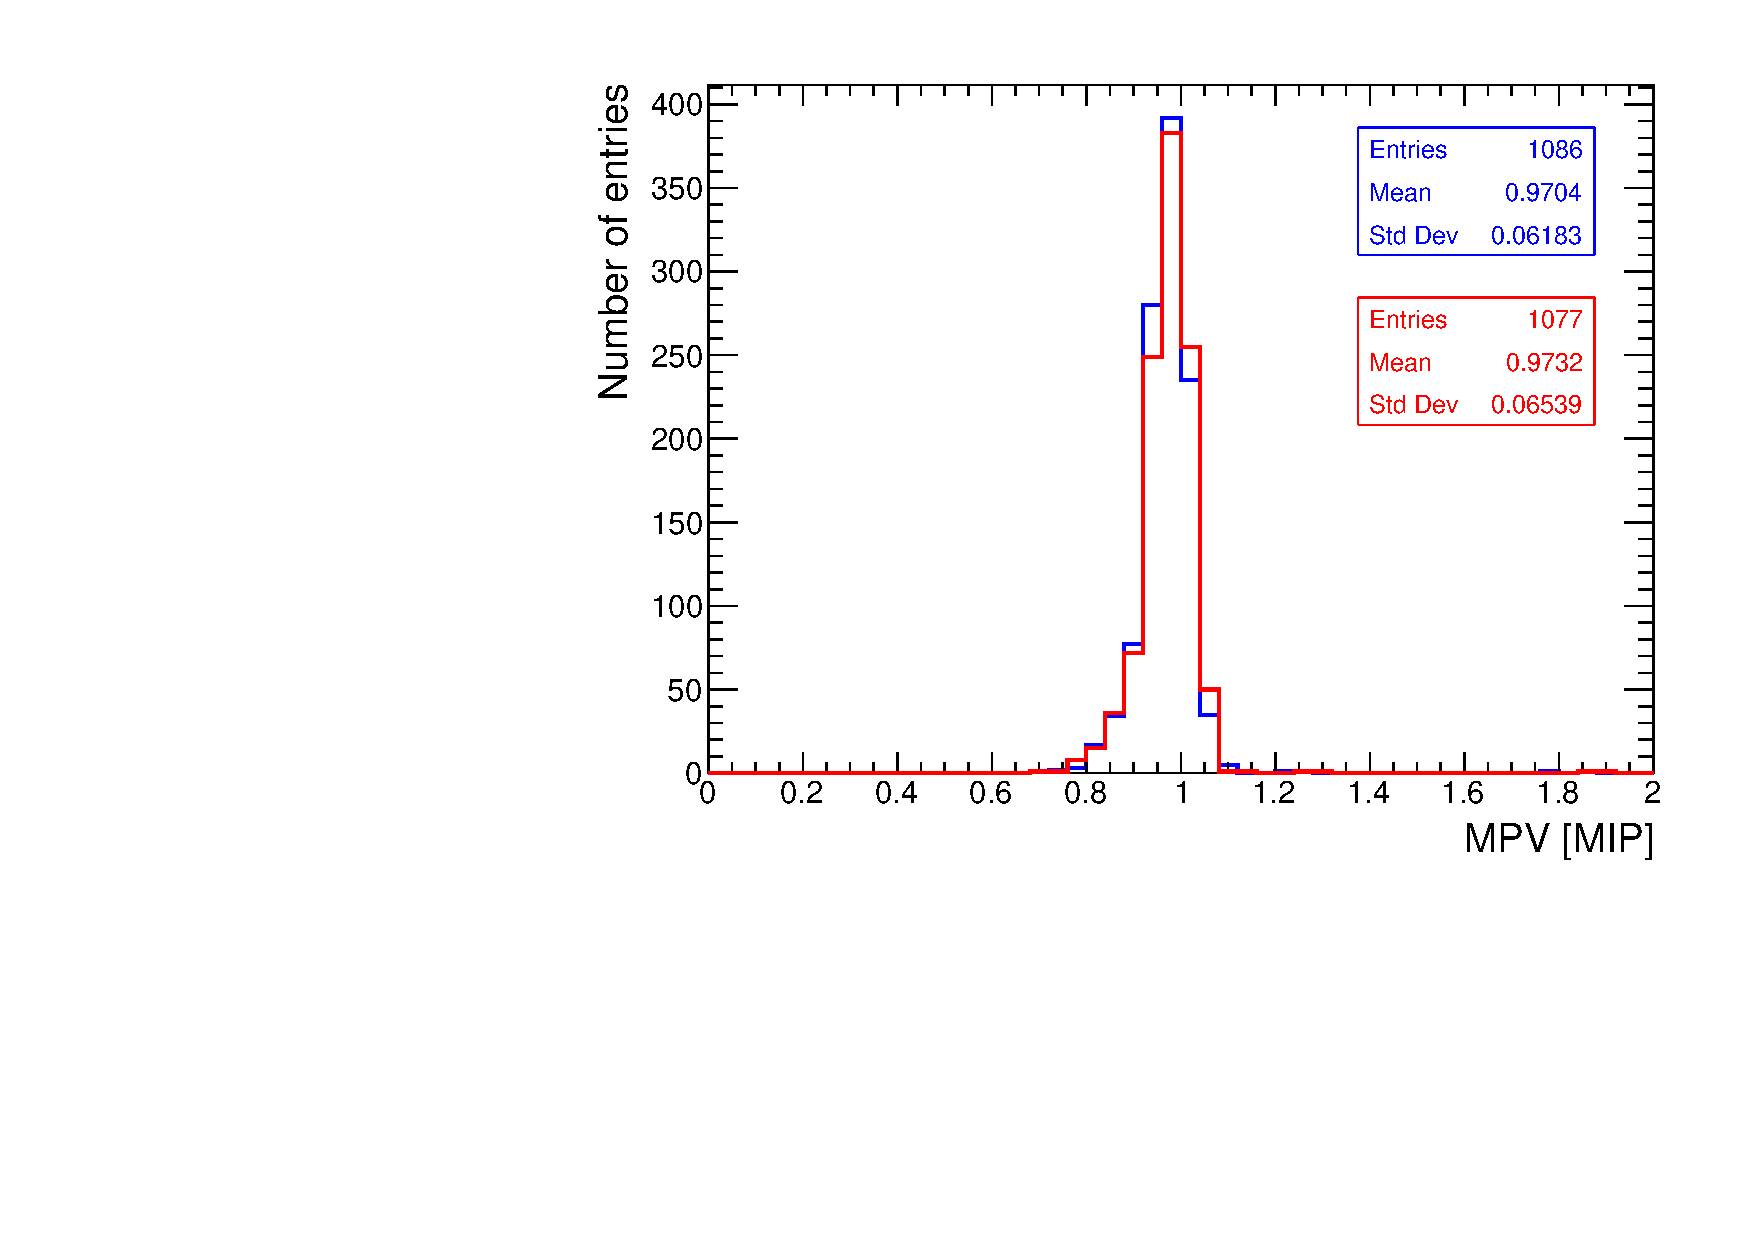
\includegraphics[width=0.6\linewidth]{../Thesis_Plots/EnergyCalib/Plots/SystematicMIP.pdf}
	\caption{MPV fitted value in MIP for the two muon sub-samples. Even runs are in blue, odd runs are in red.} \label{fig:MIPSyst}
\end{figure}

The sub-samples are very similar with a shift in the mean value of less than 1\%. A slight shoulder is present to higher MIP values though the mean is still very close to unity. By looking at the mean of the RMS of the distributions, a systematic uncertainty of around 3.6\% on the MIP energy scale can be derived. This systematic uncertainty can then be used in the timing analysis described in the next chapters.

\section{Validation of the simulation}
\label{sec:SimulationVal}

The MIP scale is crucial to the timing studies, that the simulation is validated in the following text in order to ensure its description of the data. This section first describes cross-checks performed to validate the cell-wise energy calibration in data and simulation. Then, the AHCAL simulation and digitization model are validated by comparing electromagnetic shower observables from data to simulation. Comparisons using electromagnetic interactions within the AHCAL are preferred as these interactions should be well described in simulations and are less subject to modeling uncertainties than hadronic showers.

\subsection{Beam profiles}

To simulate beam particles, the simulation is using the position and width of a particle gun as parameter. It has to be placed in x, y directions such that the beam sizes of the experiment are modeled. This is done to guaranty that the same cells of the detector are hit in data and simulation. Otherwise, this would result in a significant bias in the comparison of data and simulation. In the z-direction, the beam gun needs to be put as close as possible to the detector to avoid beam broadening by scattering on air molecules.

The best method to estimate the beam profile for data would be to analyze the beam profile provided by the wired chambers. Unfortunately, this data could not be added to the AHCAL data acquisition system. As a workaround, the mean and RMS of the center of gravity distributions in x and y are used to estimate the beam size instead. This does not reflect the true positions since both positions are biased by dead and noisy channels. The center of gravity is calculated as the following:
\begin{equation}
	CoG_x [mm] = \frac{\Sigma_i E_i x_i}{\Sigma_i E_i} \quad \text{,} \quad CoG_y [mm] = \frac{\Sigma_i E_i y_i}{\Sigma_i E_i} \quad \text{and} \quad CoG_z [mm] = \frac{\Sigma_i E_i z_i}{\Sigma_i E_i}
\end{equation}
where $E_i$ is the energy of the i-th hit and $x_i$ and $y_i$ are the x and y position of the i-th hit.

For muon runs, a flat beam profile with a half-width of 20 cm is configured in the simulation. A perfect representation of the beam profile for muons is not expected to have an impact on the MIP response in the simulation.

For electron runs, the distribution of the center of gravity in x and y directions are used as an estimate of the beam profile. The figure \ref{fig:BPe} shows the beam profiles in the x and y directions in data and simulation for 10 GeV electrons. The agreement looks good between data and simulation. This has been check for all energies. The agreement gets worse for higher electrons energies that may be due to a contamination from lower energy electrons \cite{AmbraEnergy}. In addition, at higher energy, the beam looks less gaussian-like and the shape in simulation can't be simulated perfectly.

\begin{figure}[htbp!]
	\centering
	\begin{subfigure}[t]{0.49\textwidth}
		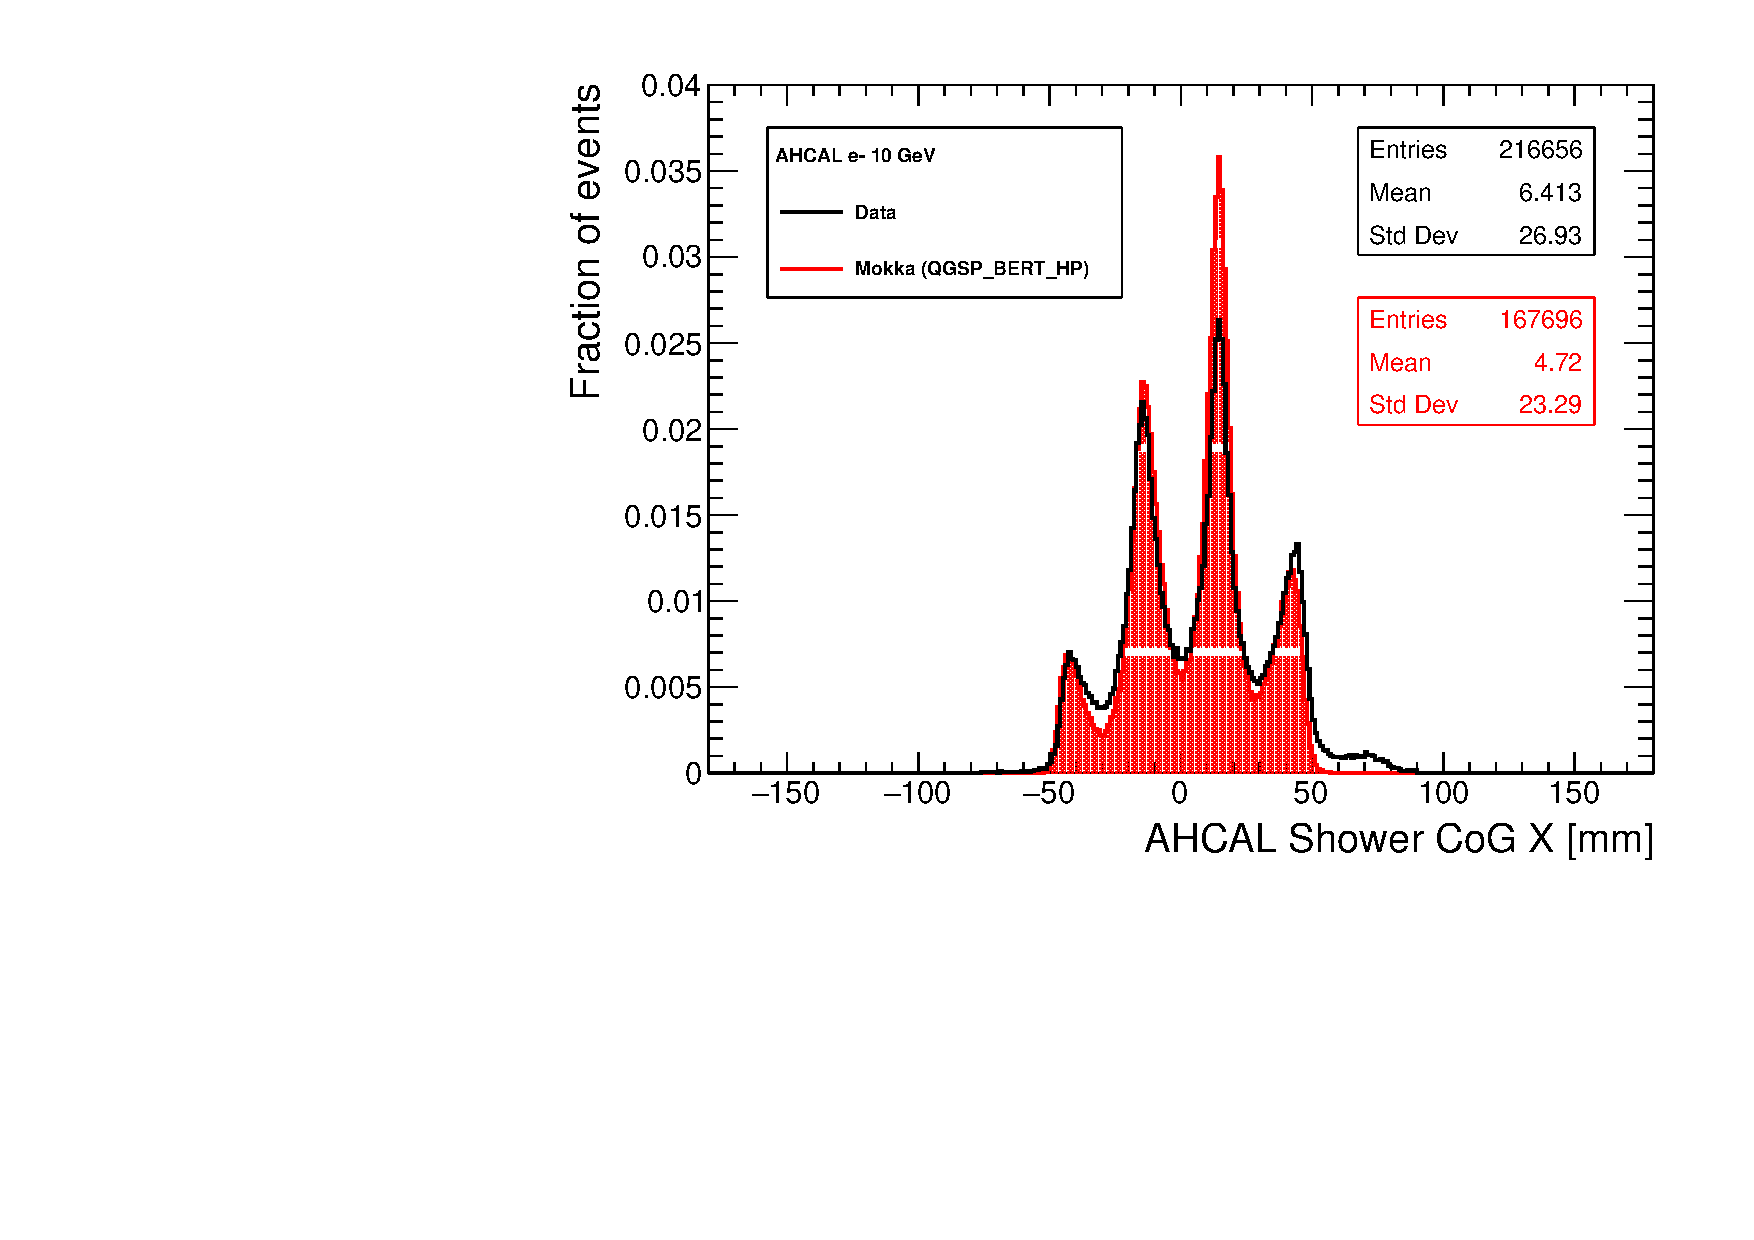
\includegraphics[width=1.\linewidth]{../Thesis_Plots/Timing/Electrons/Plots/Run24542_CoGX_AHCAL_10GeV_Comparison.pdf}
		\caption{Beam profile X.} \label{fig:e10GeVX}
	\end{subfigure}
	\hfill
	\begin{subfigure}[t]{0.49\textwidth}
		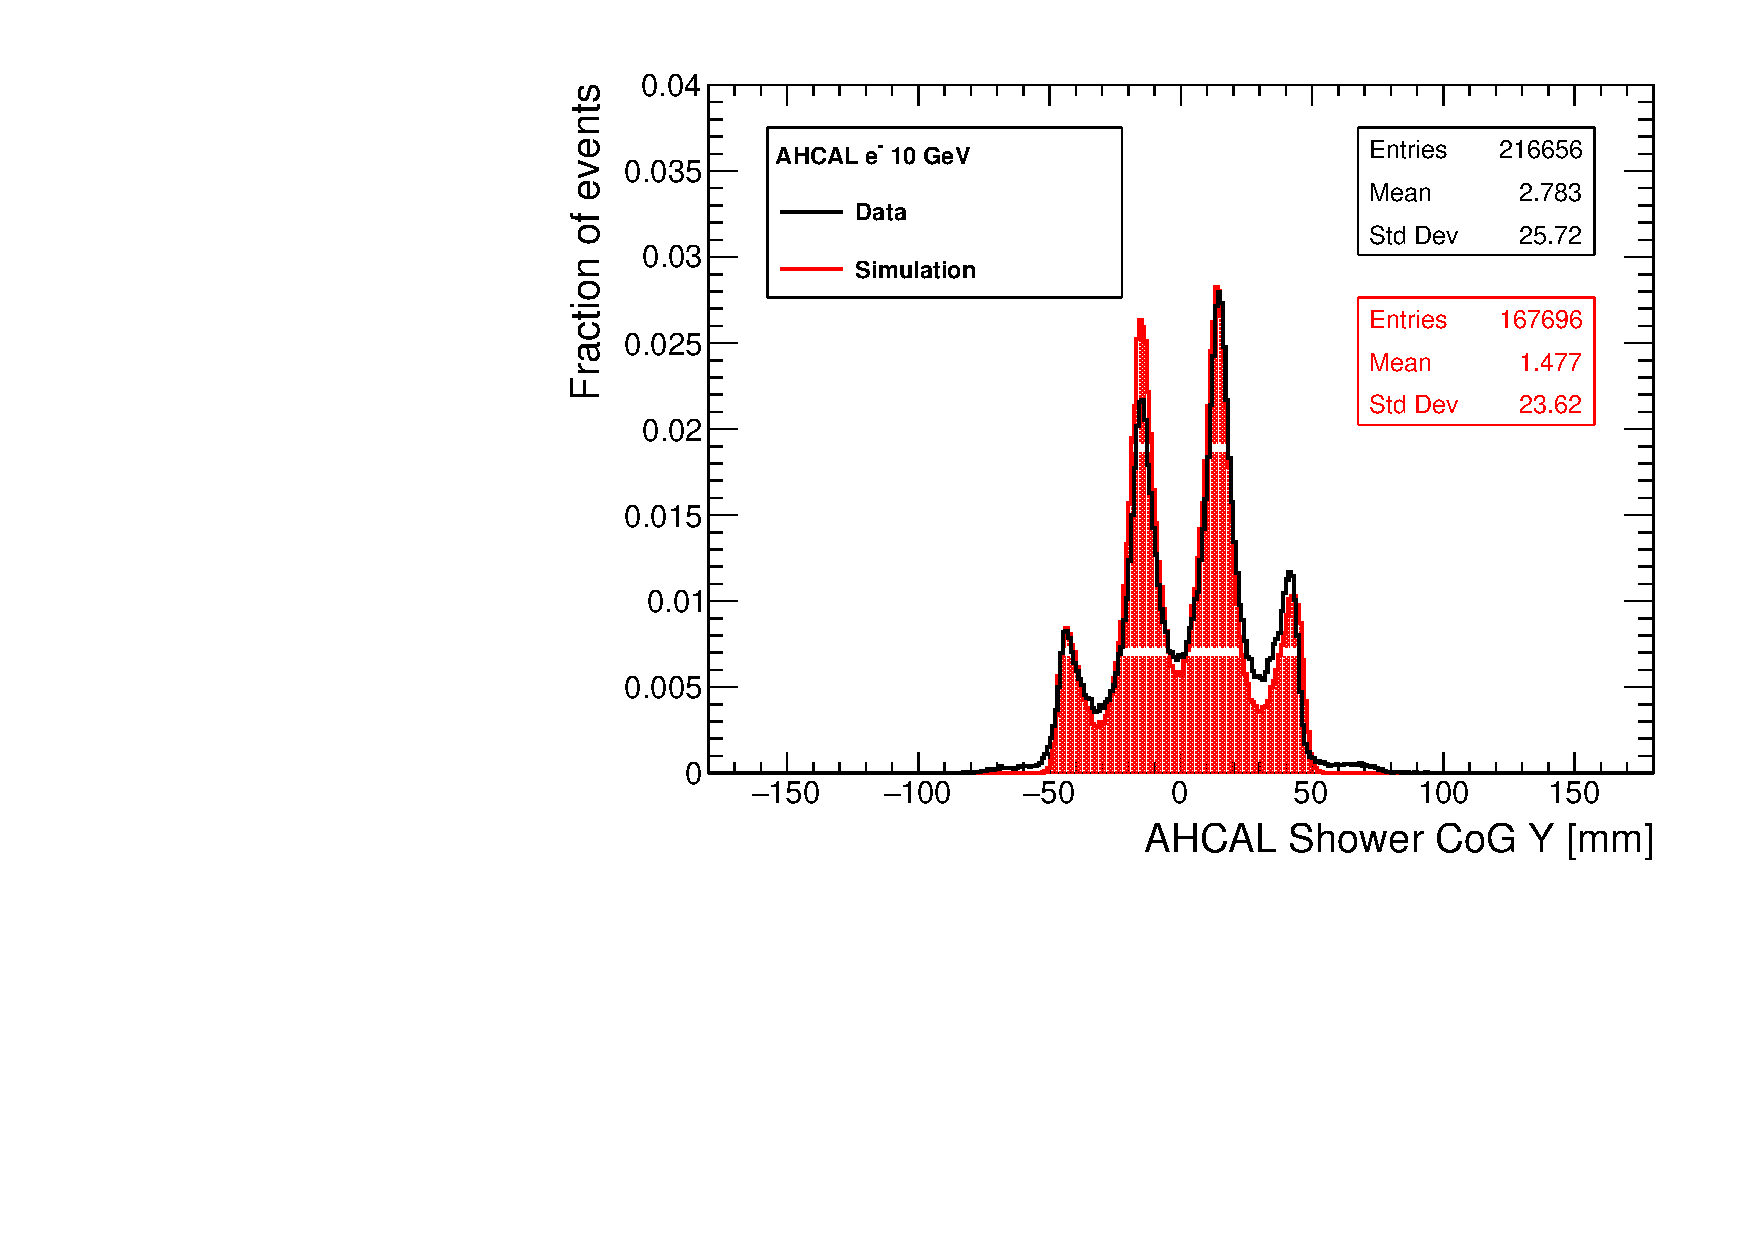
\includegraphics[width=1.\linewidth]{../Thesis_Plots/Timing/Electrons/Plots/Run24542_CoGY_AHCAL_10GeV_Comparison.pdf}
		\caption{Beam profile Y.} \label{fig:e10GeVY}
	\end{subfigure}
	\caption{Beam profiles for 10 GeV electrons in data and simulation. Simulated with QGSP\_BERT\_HP using \geant v10.1.}
	\label{fig:BPe}
\end{figure}

For pion runs, the same method as for electron runs is used. The figures \ref{fig:BPpi} show the beam profiles in the x and y-direction in data and simulation for 10 GeV pions. The agreement looks quite good for 10 GeV, with only a slight difference that is visible in the y-direction. The beam profiles have been checked also for all energies with the same conclusion.

\begin{figure}[htbp!]
	\centering
	\begin{subfigure}[t]{0.49\textwidth}
		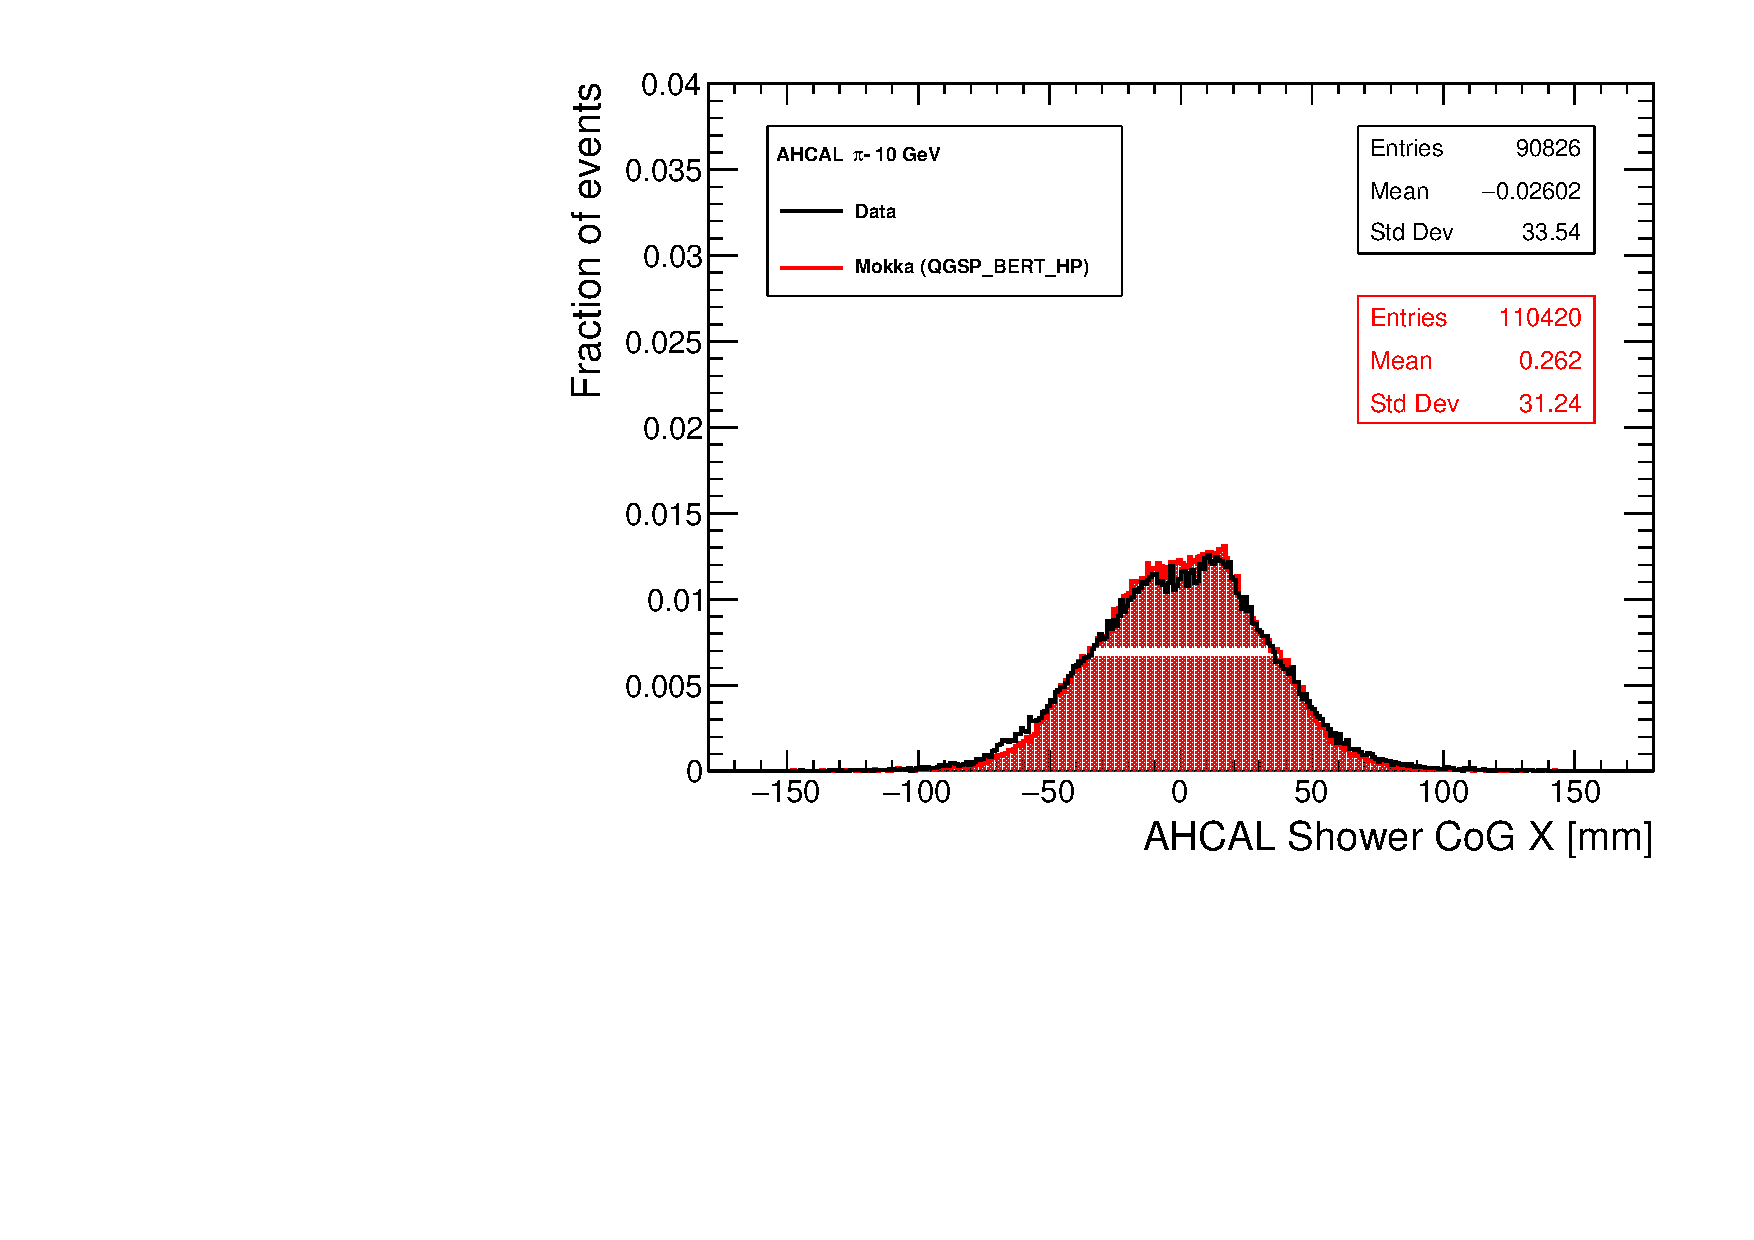
\includegraphics[width=1.\linewidth]{../Thesis_Plots/Timing/Pions/Plots/Run24306_CoGX_AHCAL_10GeV_Comparison.pdf}
		\caption{10 GeV.} \label{fig:pi10GeVX}
	\end{subfigure}
	\hfill
	\begin{subfigure}[t]{0.49\textwidth}
		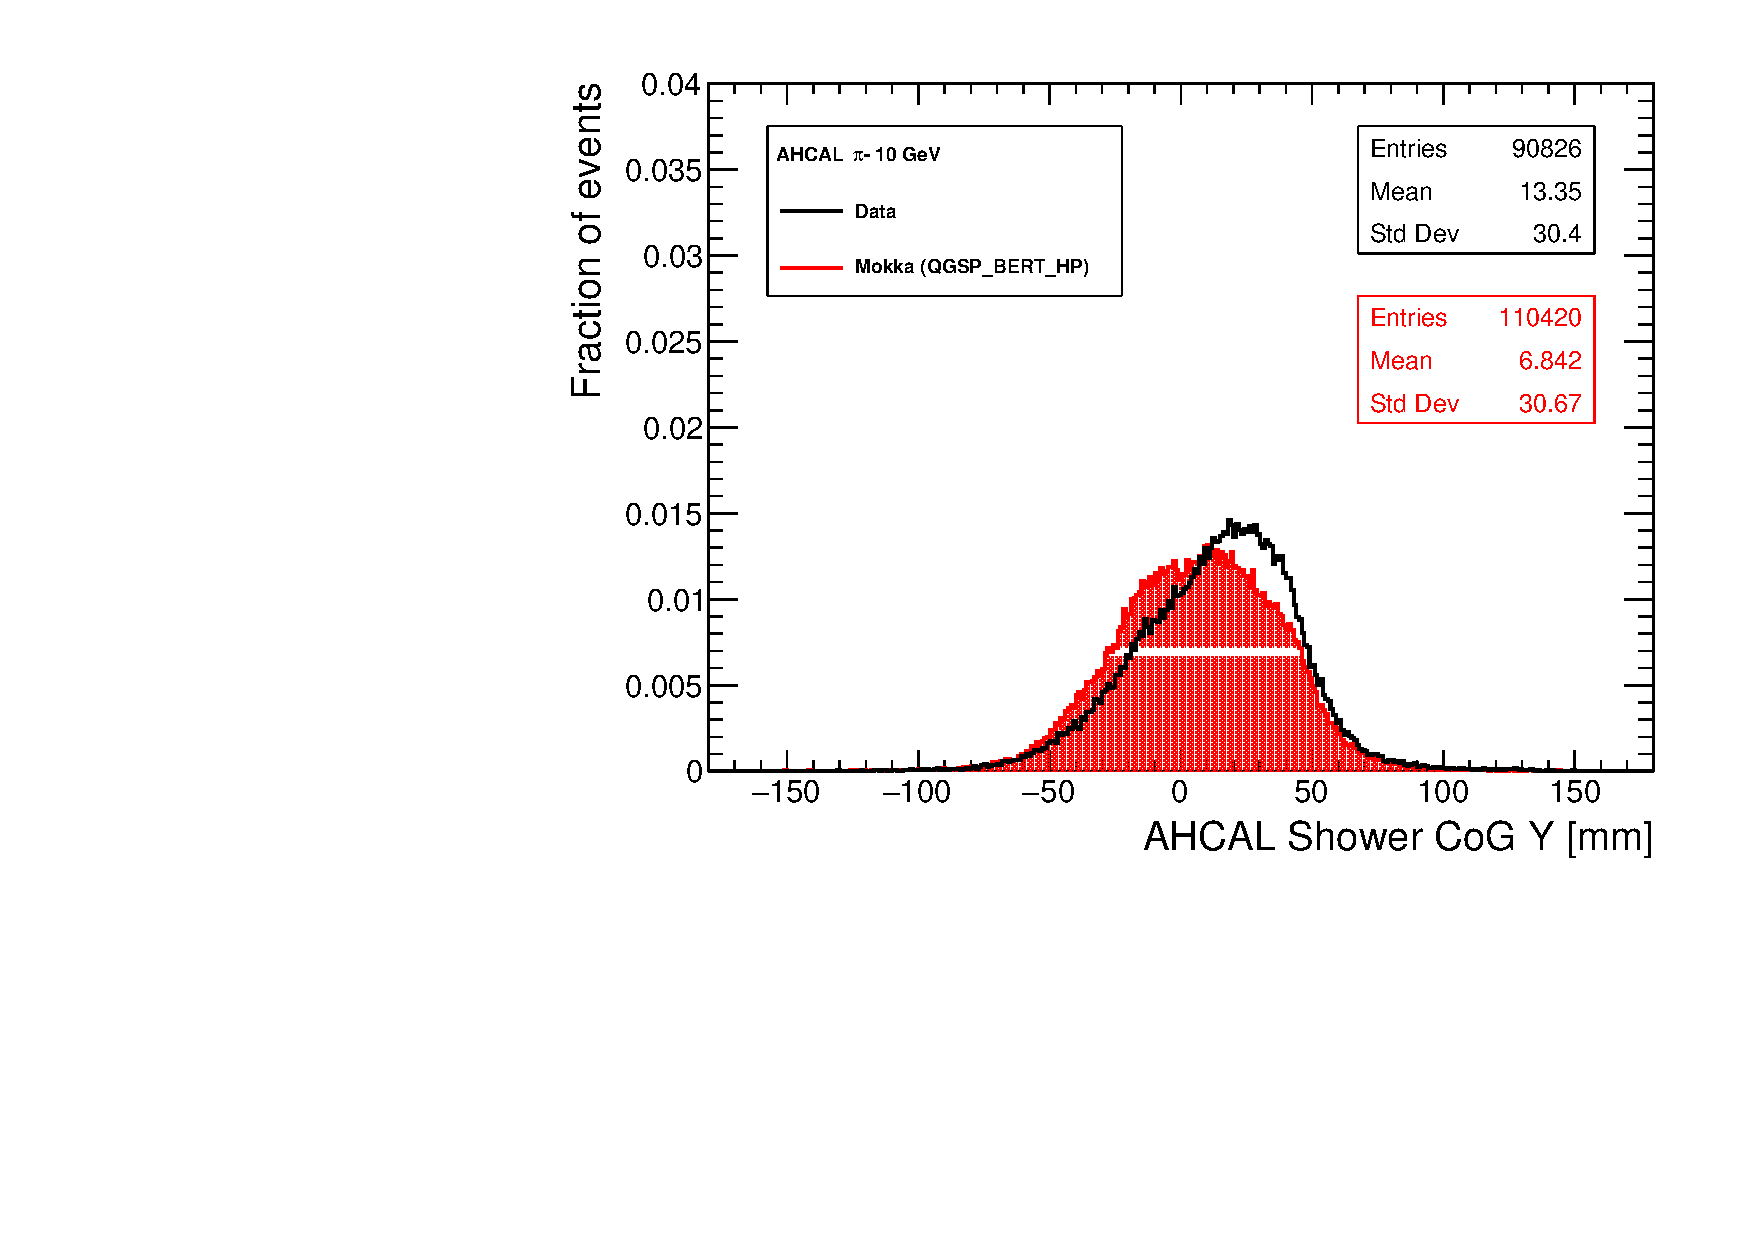
\includegraphics[width=1.\linewidth]{../Thesis_Plots/Timing/Pions/Plots/Run24306_CoGY_AHCAL_10GeV_Comparison.pdf}
		\caption{10 GeV.} \label{fig:pi10GeVY}
	\end{subfigure}
	\caption{Beam profiles for 10 GeV pions in data and simulation. Simulated with QGSP\_BERT\_HP using \geant v10.1}
	\label{fig:BPpi}
\end{figure}

Additional beam profiles can be seen in appendix \ref{appendix:SimulationVal}. The particle gun configurations used to reproduce the data runs in this thesis are shown in table \ref{table:ParticleGun}.

\begin{table}[htb!]
	\centering
	\caption{Settings of the particle gun in simulation used to reproduce the beam profile of the data runs used in this thesis.}
	\label{table:ParticleGun}
	\begin{tabular}{@{} lcccccc @{}}
		\toprule
		Type & Energy [GeV] & $\sigma_{E}$ [GeV] & $\mu_{x}$ [mm] & $\mu_{y}$ [mm] & $RMS_{x}$ [mm] & $RMS_{y}$ [mm] \\
		\midrule
		$e^-$ & 10 & 0.2 & 7.5 & 3.2 & 29.2 & 27.5\\
		$e^-$ & 15 & 0.3 & 5.6 & 2.9 & 28.0 & 26.2\\
		$e^-$ & 20 & 0.4 & 2.1 & -0.3 & 27.0 & 26.1\\
		$e^-$ & 30 & 0.6 & -4.6 & 18.5 & 23.8 & 21.9\\
		$e^-$ & 40 & 0.8 & -2.8 & 11.3 & 24.7 & 25.5\\
		$e^-$ & 50 & 1 & -18.4 & 5.8 & 28.2 & 28.9\\
		\midrule
		$\pi^-$ & 10 & 0.2 & -0.3 & 14.8 & 34.6 & 29.8\\
		$\pi^-$ & 30 & 0.6 & 7.7 & -1.9 & 28.3 & 26.4\\
		$\pi^-$ & 50 & 1 & 10.1 & 14.0 & 19.6 & 17.1\\
		$\pi^-$ & 70 & 1.4 & 21.9 & -14.5 & 28.8 & 28.6\\
		$\pi^-$ & 90 & 1.8 & 3.2 & 2.8 & 23.7 & 23.5\\
		\bottomrule
	\end{tabular}
\end{table}

\subsection{MIP Calibration}

The MIP calibration defines the energy scale of the energy depositions measured in the AHCAL. It is needed to carefully validate the MIP calibration in data and in simulation in order to be able to compare results.

Applying the MIP selection on the muon runs results in energy depositions of single MIP amplitudes for all channels. The comparison of the MIP spectrum for the whole AHCAL between data and simulation is shown in figure \ref{fig:MIPData_MC}. The shape of the hit energy spectrum matches relatively well. The data appears slightly wider than for simulation because of channel-by-channel mis-calibrations that are not modeled in the simulation. The figure \ref{fig:muEdep} shows the mean energy deposition per layer. The simulation reproduces the data within 3-4\%. This comparison validates the simulation at the lowest hit energies.

\begin{figure}[htbp!]
	\centering
	\begin{subfigure}[t]{0.49\textwidth}
		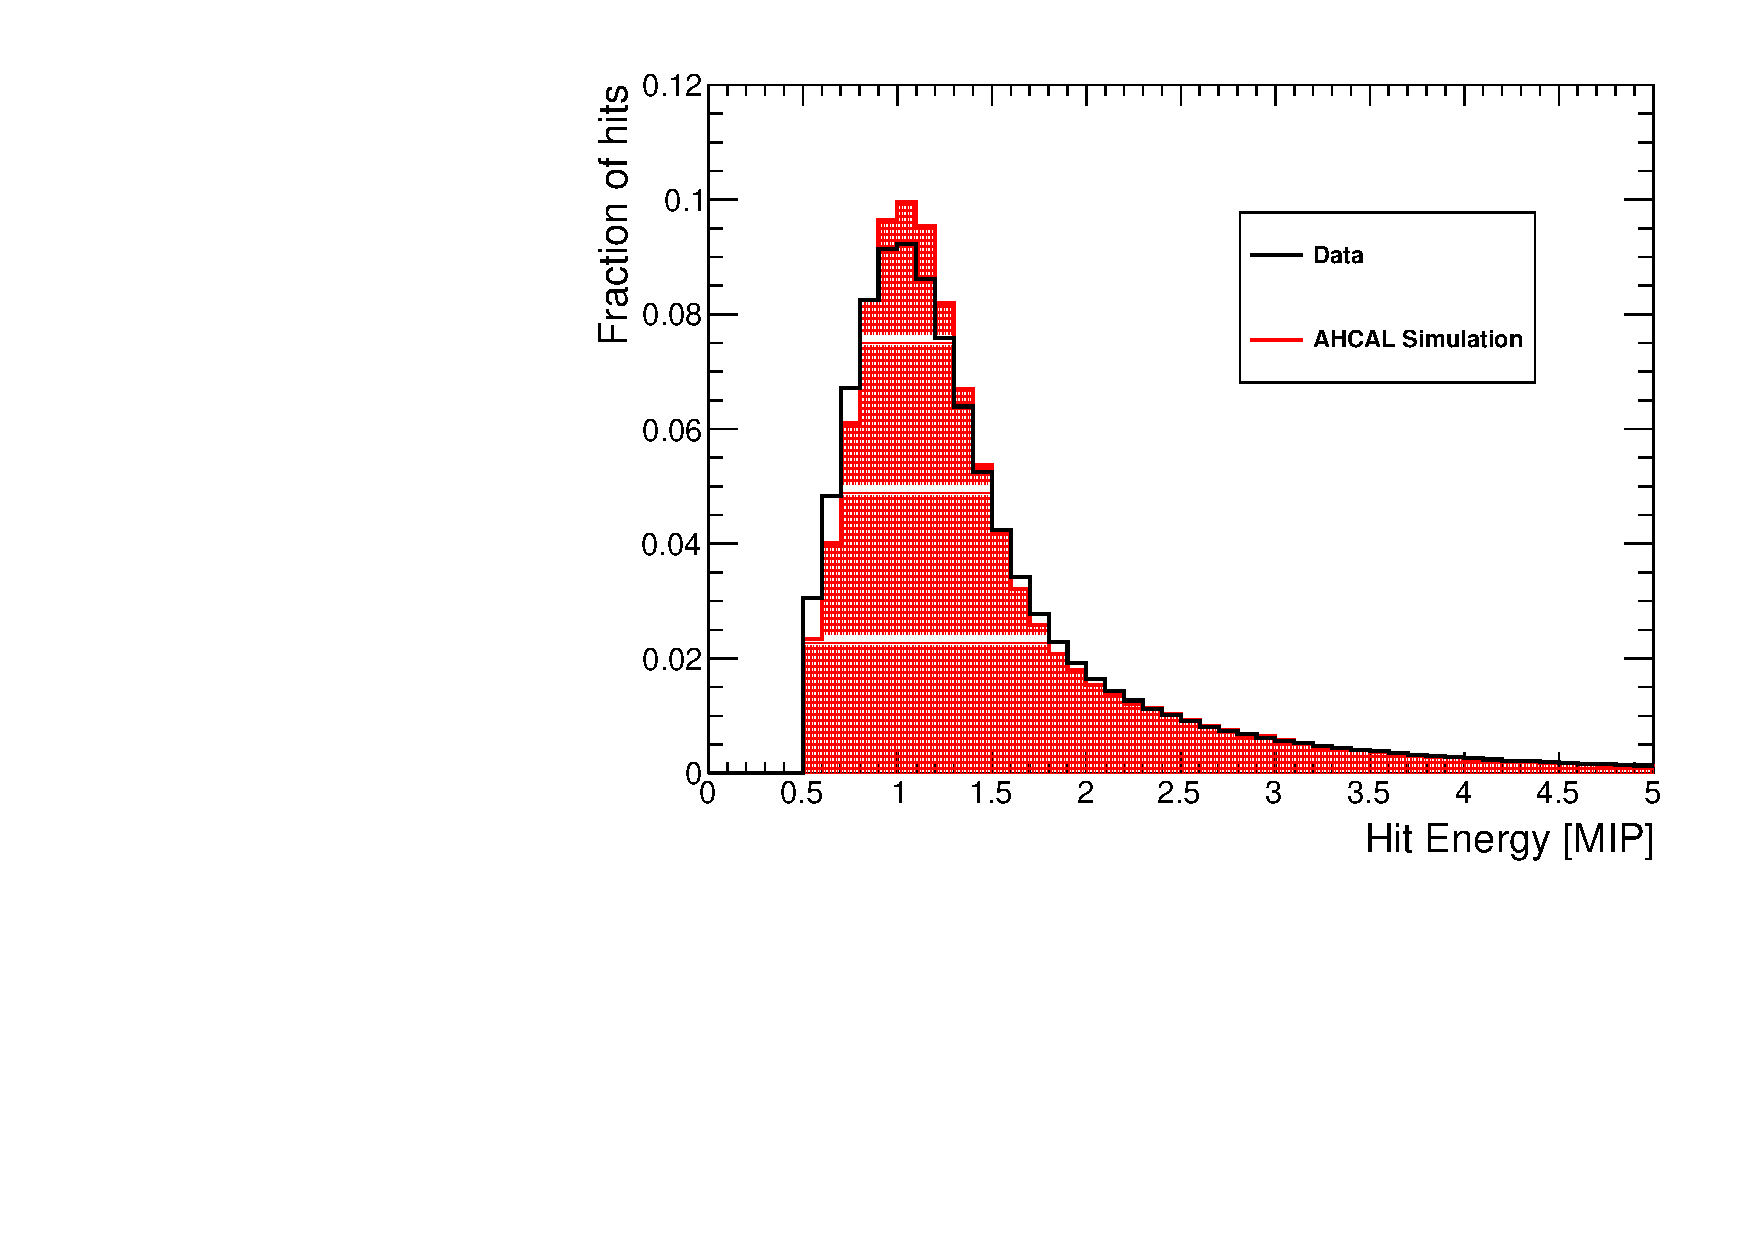
\includegraphics[width=1\linewidth]{../Thesis_Plots/EnergyCalib/Plots/ComparisonMCData_MIPPeak.pdf}
		\caption{} \label{fig:MIPData_MC}
	\end{subfigure}
	\hfill
	\begin{subfigure}[t]{0.5\textwidth}
		\centering
		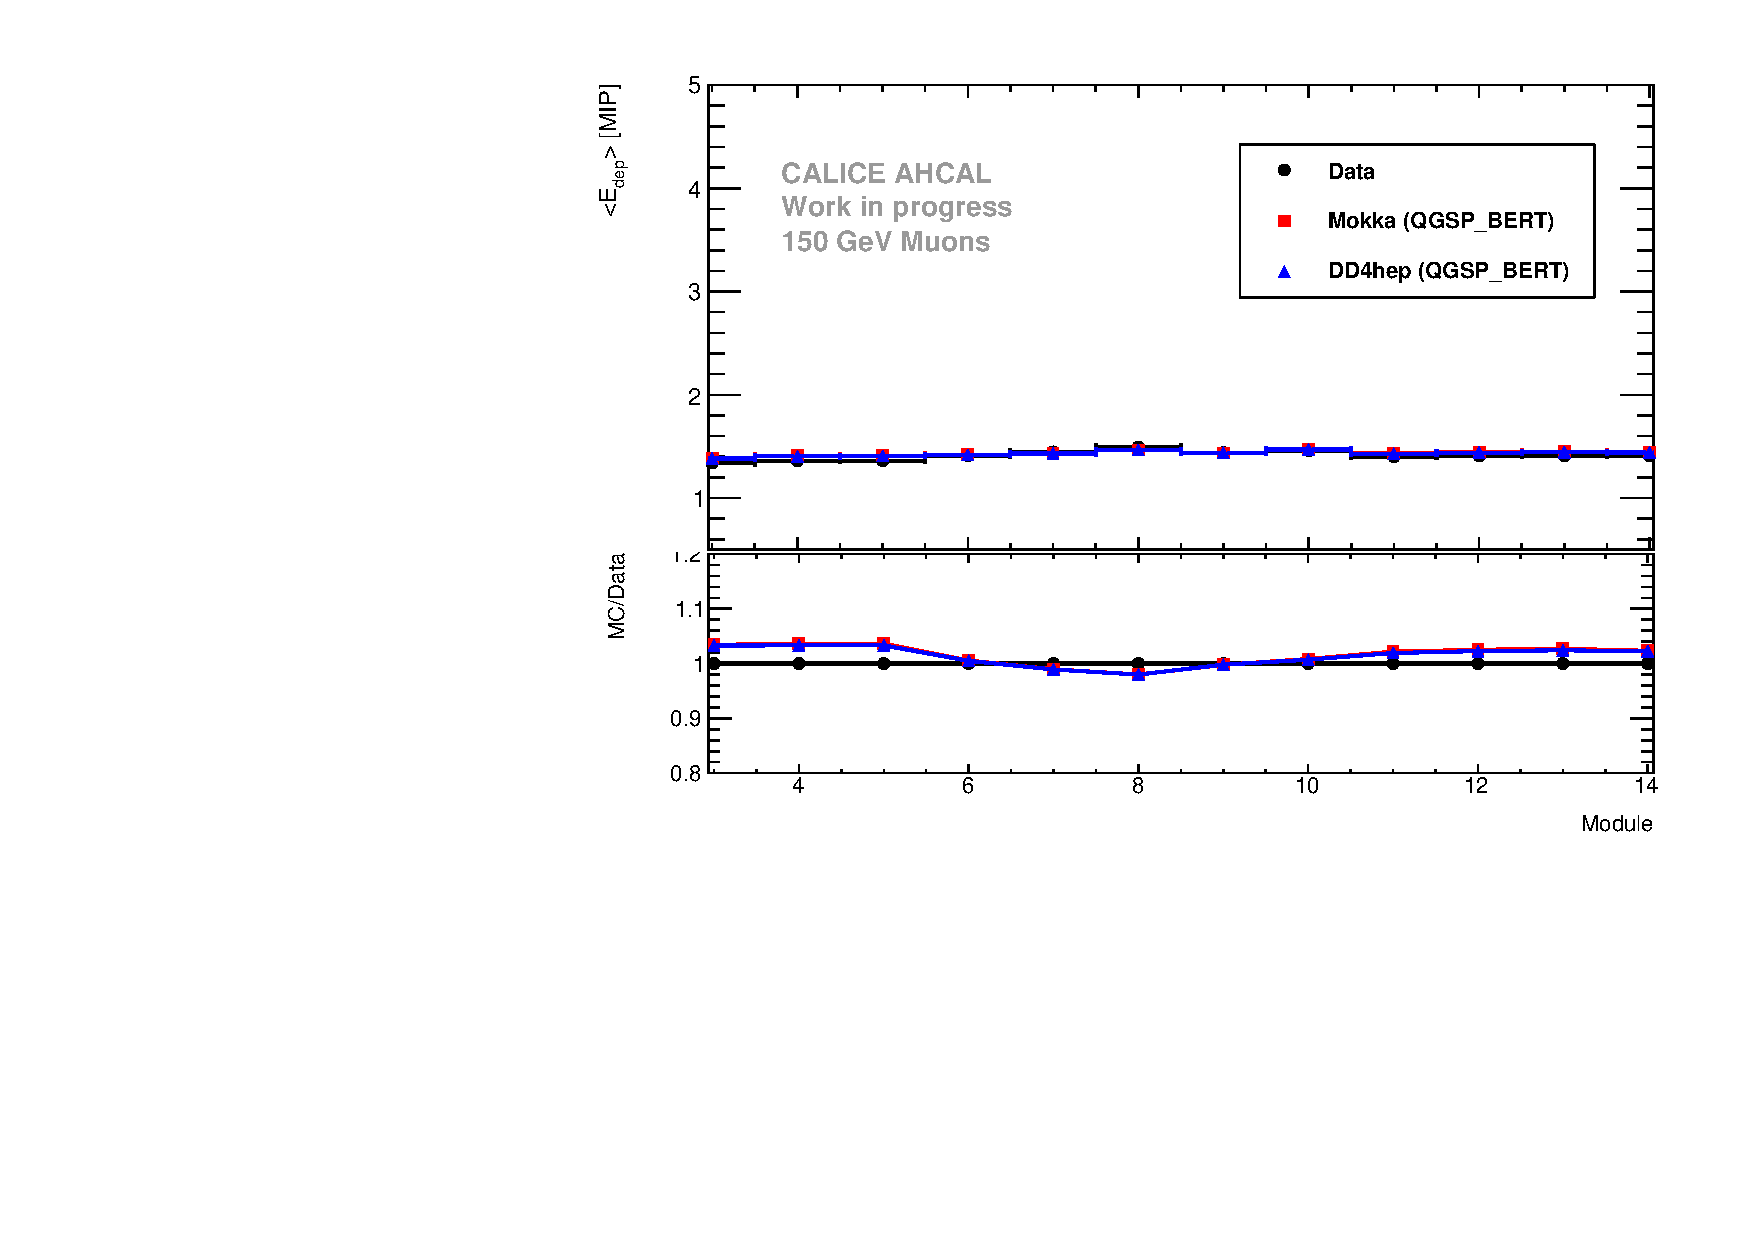
\includegraphics[width=1\linewidth]{../Thesis_Plots/Timing/Muons/Plots/ProfileMuons_Edep.pdf}
		\caption{} \label{fig:muEdep}
	\end{subfigure}
	\caption{\subref{fig:MIPData_MC}) Hit Energy Spectra for the complete AHCAL for muon like-track hits for both data and simulation. \subref{fig:muEdep}) Longitudinal mean energy profile for muon like-track hits in data and simulations.}
	\label{fig:Val}
\end{figure}

The figure \ref{fig:MPVData_MC} shows the distribution of the extracted MIP calibration constant for single channels in data and simulation. Ideally, the distribution should peak at the unity for all channels. But in practice, due to the fitting procedure uncertainty, mis-calibrations and statistic limitation, it results in a widening of the distribution. Both data and simulation give a mean value around 1 MIP for the AHCAL indicating a good average calibration at the cell level. The higher values to the right that appear in the data have been checked and all channels present a good fit. The AHCAL simulation is slightly shifted to the right to higher values but is still reasonably close to unity.

\begin{figure}[htbp!]
	\centering
	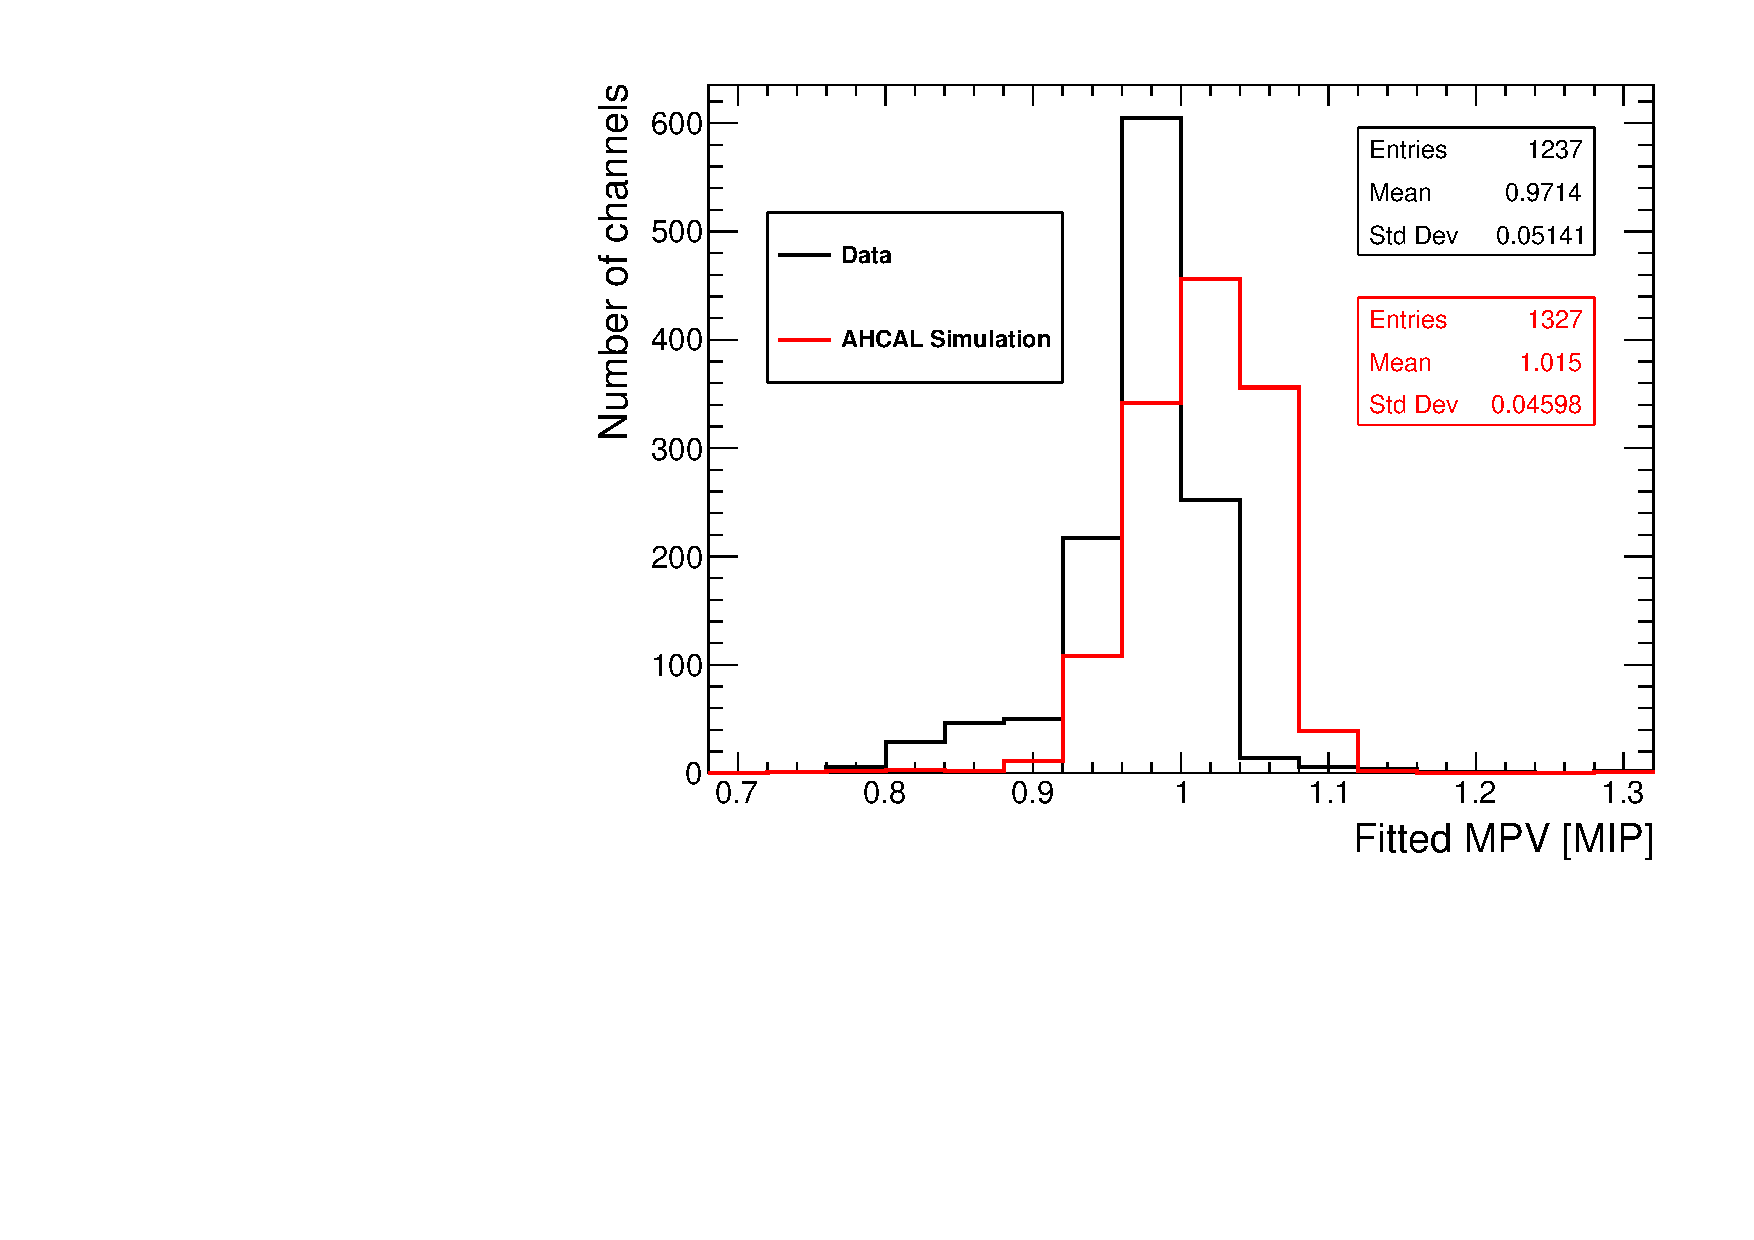
\includegraphics[width=0.6\linewidth]{../Thesis_Plots/EnergyCalib/Plots/ComparisonMCData_MPV.pdf}
	\caption{Distribution of the fitted MIP value in single channels of the AHCAL for data and simulation.} \label{fig:MPVData_MC}
\end{figure}

\subsection{Electrons}

Electromagnetic showers are used to validate further the simulation. As the physics of electron showers are very well understood and can be simulated with great accuracy, it is used as a tool to validate the detector geometry, especially concerning the material composition as well as the general calibration. Besides noise and beam profiles, the influence of cross-talk has a significant impact due to the higher energy deposited.

In addition, the SiPM saturation unfolding of high energy cells is very important as generally electrons deposit in few cells all their energy. Unfortunately, no saturation curves are available and only estimations of the necessary parameters are used. However, in this thesis, the energy deposited in a single cell is only relevant at low energies (from 0.5 to few MIPs) where the response of the SiPM is linear. Therefore, the SiPM saturation unfolding is not used. Only saturation of the hit energy is performed on the simulation as hits from the data are obtained saturated.

The figure \ref{fig:eHitVal} shows the hit energy spectra for 10 GeV and 50 GeV electron showers in data and simulation. Hit energies up to 60 MIPs are well described by the simulation up to 10\%. A small difference is noticeable around 20 MIPs because of overestimated intercalibration factors between high gain hits and low gain hits that shift the hit energy to slightly higher values. For 10 GeV, the simulation is underestimating the hit energy by a large factor over 60 MIPs. It is similar at higher beam energies. At 50 GeV, the region between 120 to 220 MIPs is overestimated by the simulation. The underestimation in simulation of the hit energy comes from an incorrect value of the number of effective pixels used in the saturation function (see equation \ref{eq:SiPMfunction}) to saturate hits in the simulation. This number is too small thus saturating the simulation to lower hit energies. The description of the shape of the hit energy spectra is influenced by the formula of saturation function used \cite{Kotera:2015rha} and the figure shows that for energies between 100 and 200 MIPs, the current function is not good enough to describe well the shape of the observed hit energy spectra in data.

\begin{figure}[htbp!]
	\centering
	\begin{subfigure}[t]{0.49\textwidth}
		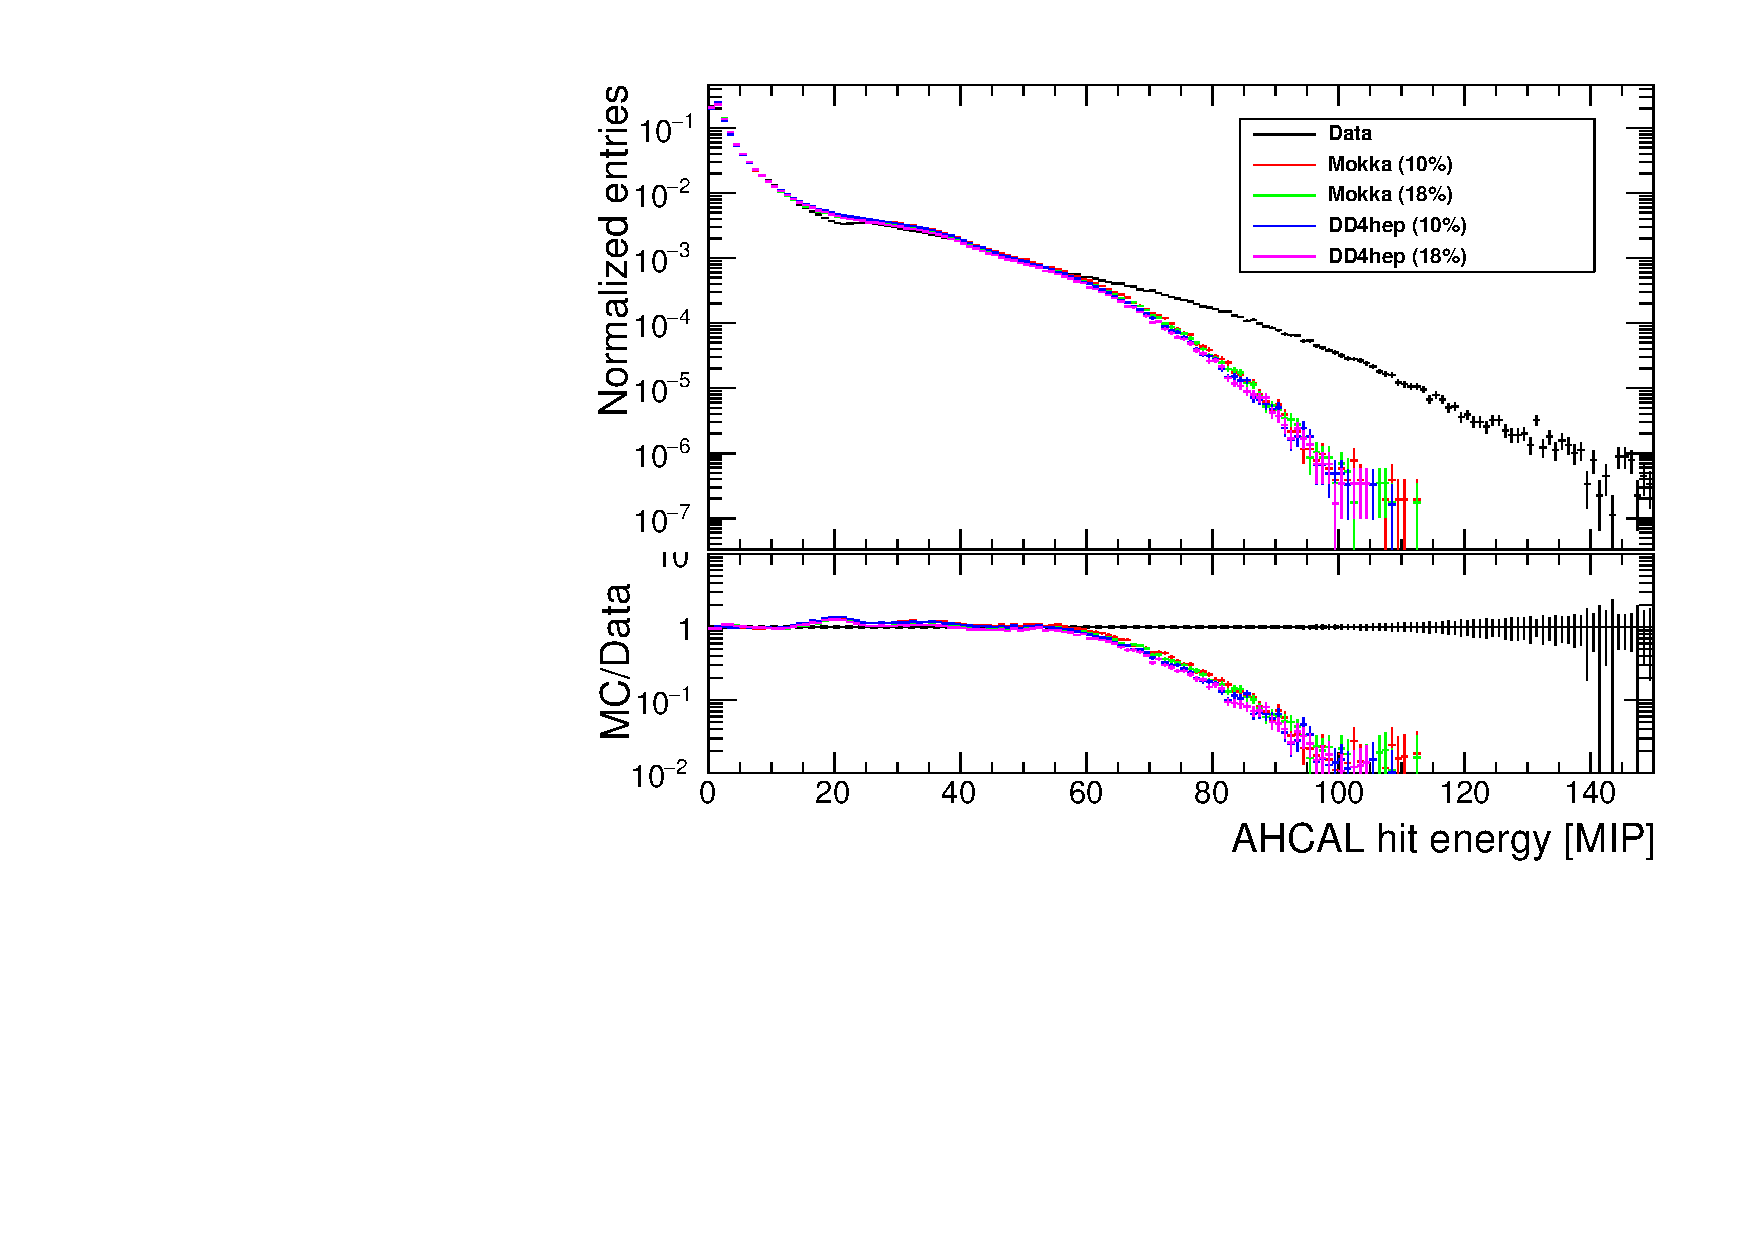
\includegraphics[width=1.\linewidth]{../Thesis_Plots/EnergyCalib/Plots/HitEnergy_Electrons10GeV.pdf}
		\caption{10 GeV} \label{fig:HitEnergy10GeVe}
	\end{subfigure}
	\hfill
	\begin{subfigure}[t]{0.49\textwidth}
		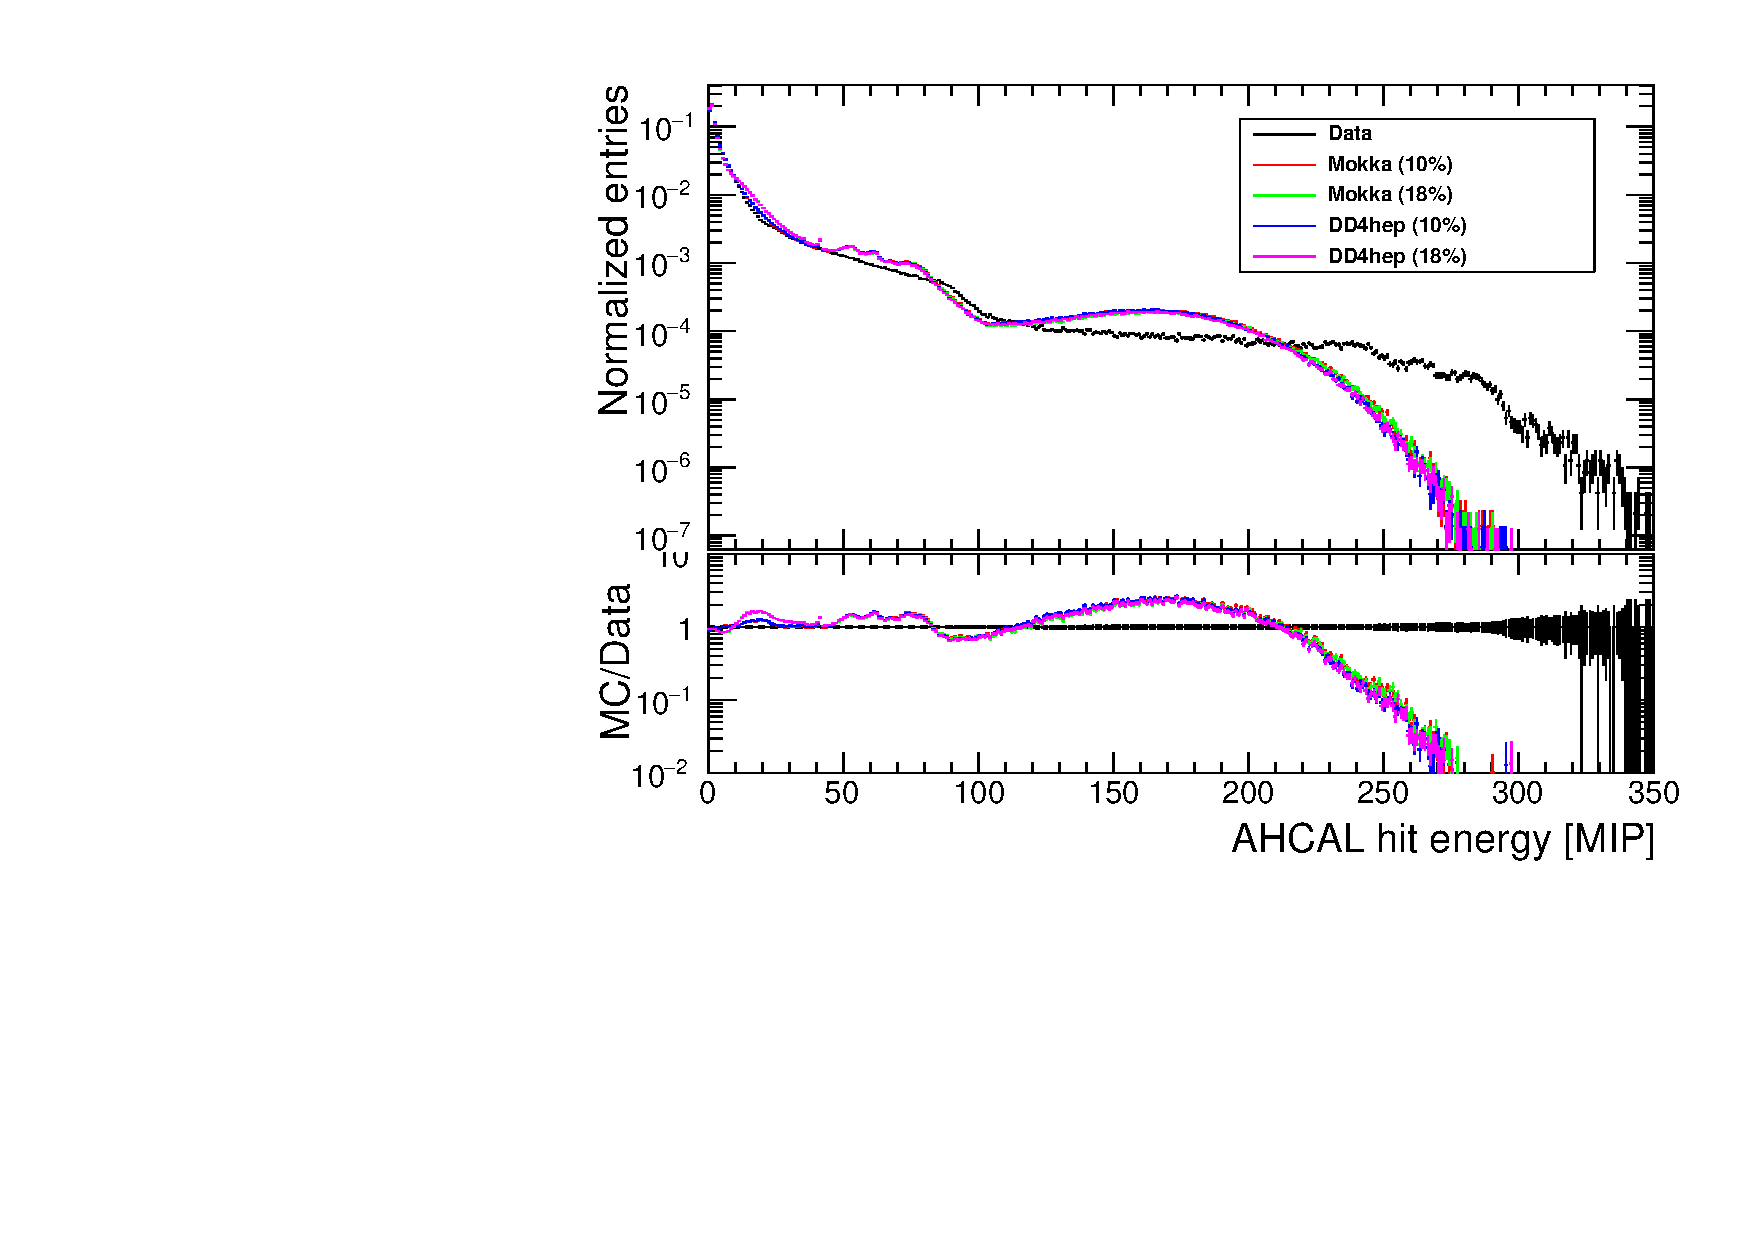
\includegraphics[width=1.\linewidth]{../Thesis_Plots/EnergyCalib/Plots/HitEnergy_Electrons50GeV.pdf}
		\caption{50 GeV} \label{fig:HitEnergy50GeVe}
	\end{subfigure}
	\caption{Electron hit energy spectra for data and simulation for 10 and 50 GeV beam energies. The different colors corresponds to the variation of the cross-talk parameter in the simulations between 10\% and 18\%.}
	\label{fig:eHitVal}
\end{figure}

The figure \ref{fig:EsumMeanElectron} show the mean energy sum $<E_{sum}>$ and figure \ref{fig:nHitsMeanElectron} shows the mean number of hits $<nHits>$ as a function of the electron beam energy between 10 and 50 GeV in data and simulation with different cross-talk parameters. The mean is obtained from the mean of the distribution, no fit is performed. The visible energy for data agrees within the simulations for 10, 15 and 20 GeV electron energy and seems to agree better with the 10\% cross-talk simulations. For higher energies, the data deviates significantly to lower values due to the presence of the long tail left of the distribution that the simulations cannot describe (see appendix \ref{appendix:SimulationVal}). The curve does not look linear as one would expect, this is probably due to saturation effects that are not corrected.

The number of hits is well described in the simulations but agrees better with 10\% cross-talk at low energies and with the 18\% cross-talk at higher energies. However, the data cannot be described for both distributions at once in either simulation with a global cross-talk parameter.

\begin{figure}[htbp!]
	\centering
	\begin{subfigure}[t]{0.49\textwidth}
		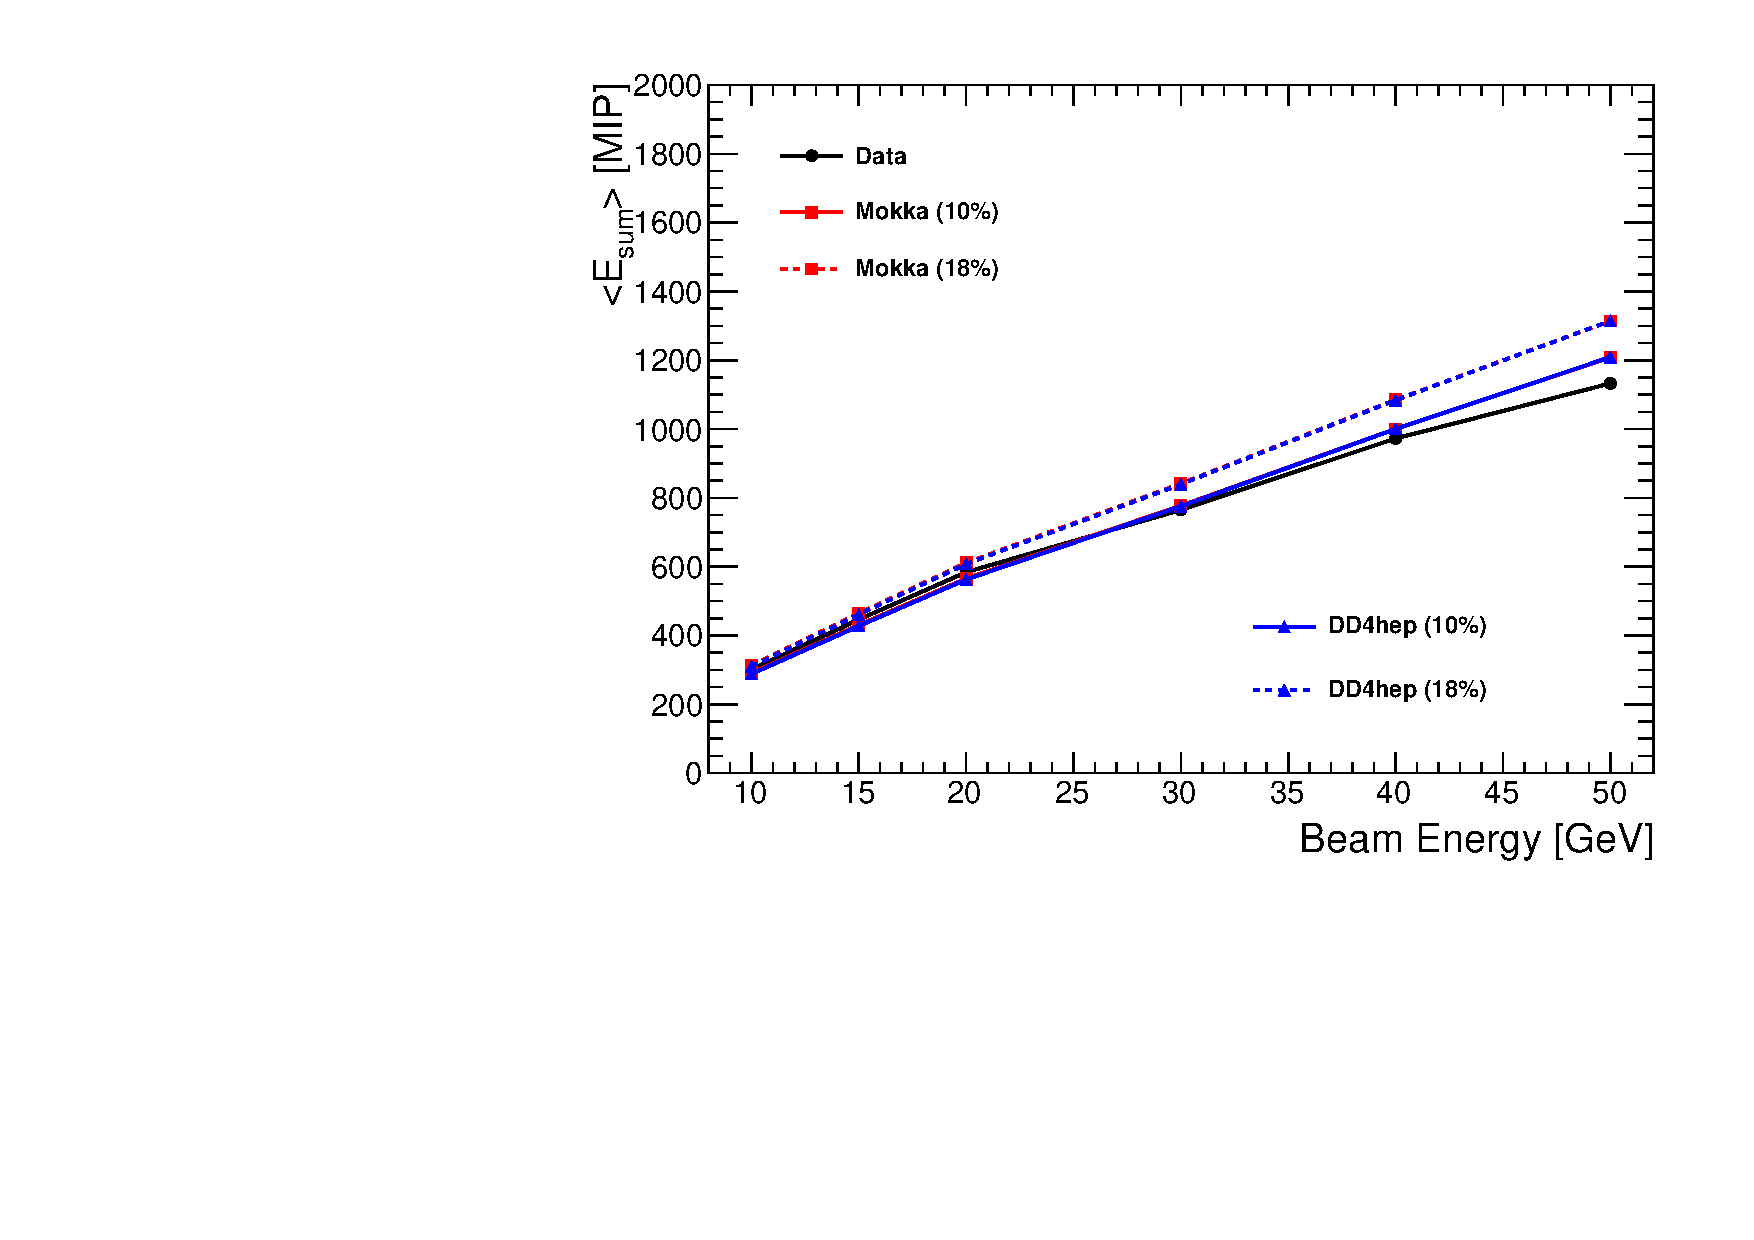
\includegraphics[width=1.\linewidth]{../Thesis_Plots/Timing/Electrons/Plots/EsumElectrons_BeamEnergy.pdf}
		\caption{} \label{fig:EsumMeanElectron}
	\end{subfigure}
	\hfill
	\begin{subfigure}[t]{0.49\textwidth}
		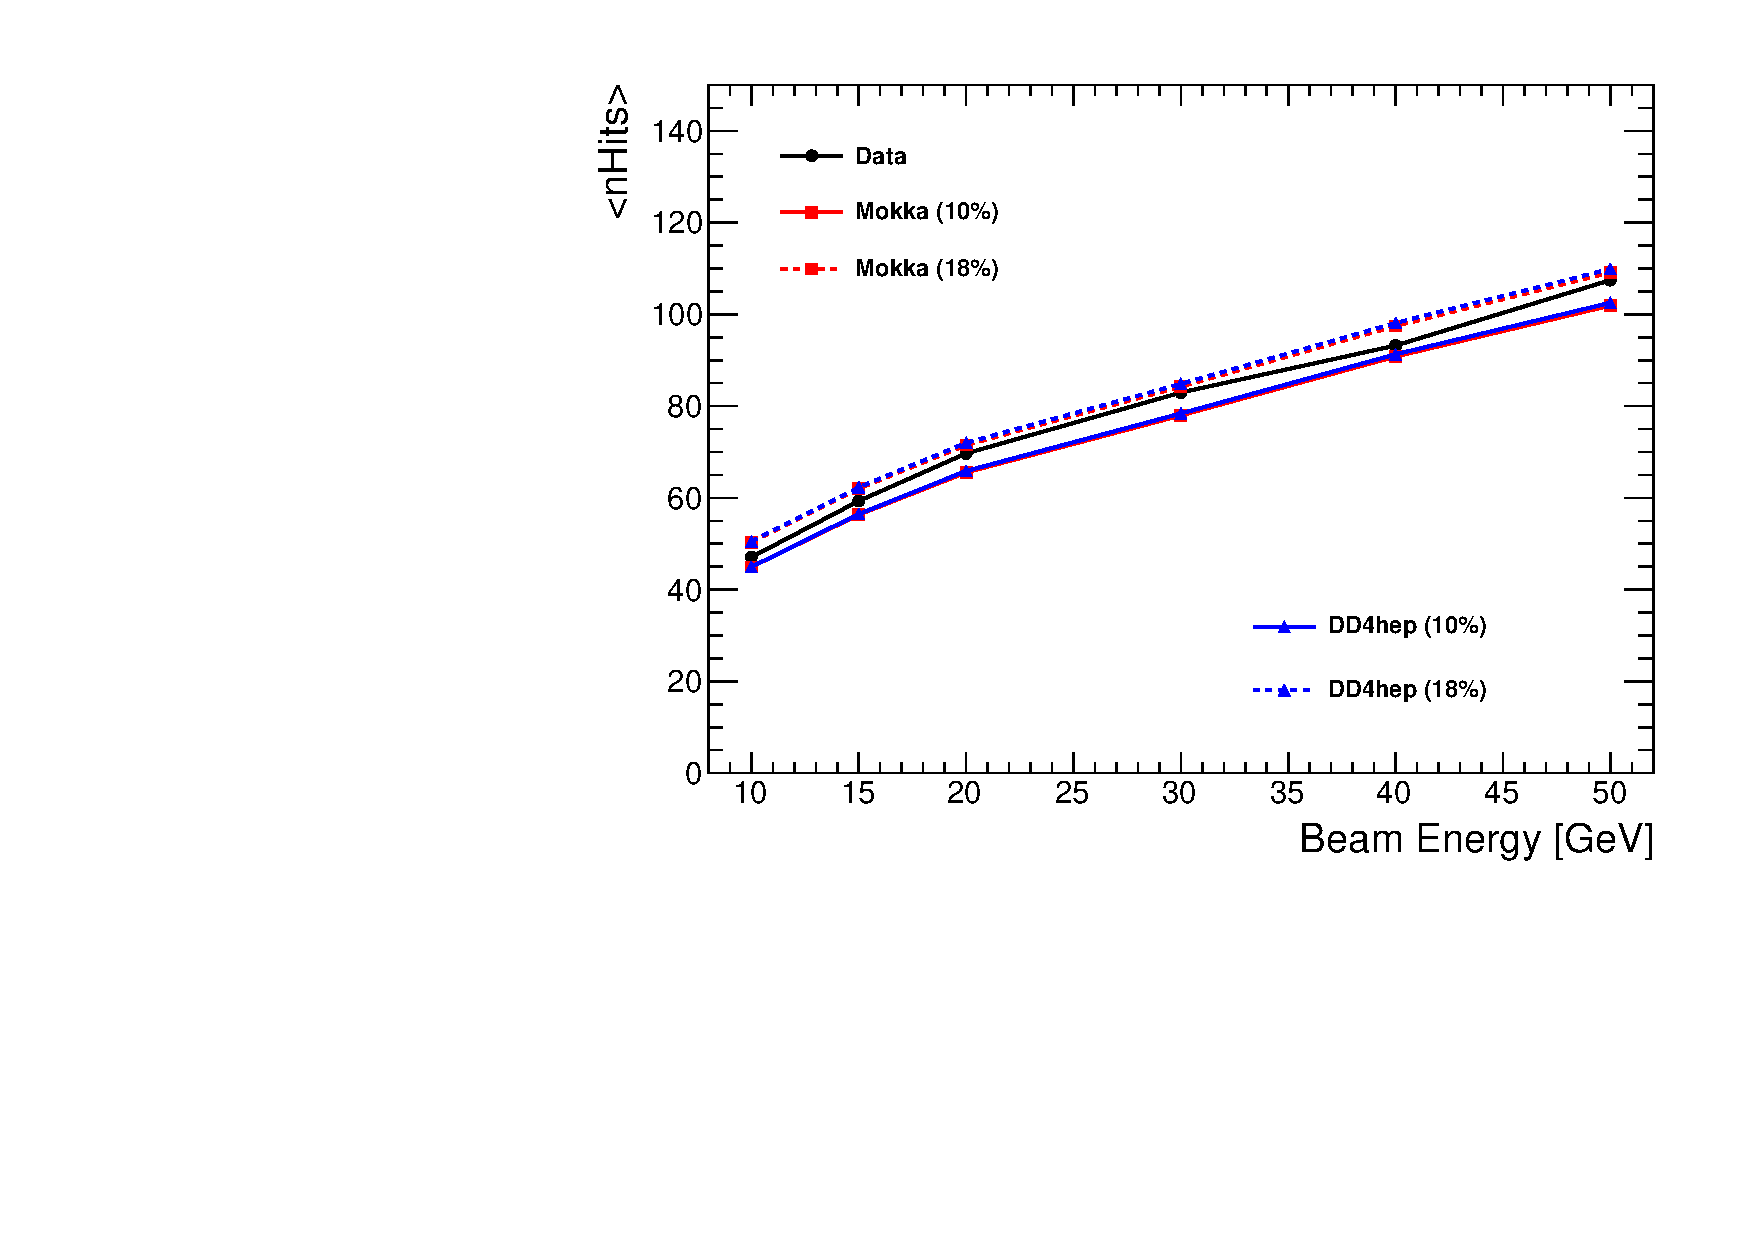
\includegraphics[width=1.\linewidth]{../Thesis_Plots/Timing/Electrons/Plots/nHitsElectrons_BeamEnergy.pdf}
		\caption{} \label{fig:nHitsMeanElectron}
	\end{subfigure}
	\caption{\subref{fig:EsumMeanElectron}) Comparison of the mean energy sum in the AHCAL as function of the beam energy for electron data and simulations with different cross-talk parameters. Simulated with QGSP\_BERT\_HP in \geant v10.1. \subref{fig:nHitsMeanElectron}) Comparison of the mean number of hits in the AHCAL as function of the beam energy for electron data and simulations with different cross-talk parameters. Simulated with QGSP\_BERT\_HP in \geant v10.1.}
	\label{fig:eVal}
\end{figure}

The precision of the detector simulation for electrons is limited by the cross-talk simulation. For energies above 20 GeV, the possible contamination with low energy electrons in the data limits as well the agreement between data and simulation. A deeper investigation on the energy aspect of the data is carried out in parallel of this analysis \cite{AmbraEnergy}. The description of electromagnetic showers in simulations is satisfactory for the study of the time development of hadron showers.

\begin{center}
	\rule{0.5\textwidth}{.4pt}
\end{center}

The MIP calibration procedure was explained and developed in order to accommodate to such high number of channels as well as the diversity in SiPM types and tile designs. In this way, 85\% of the 3744 channels in the detector have their MIP constant determined. An error around 1-3\% is made on the MIP constant value with the current fitting method which is in the order of magnitude expected due to the limited statistics. In order to validate the calibration and the simulation model, comparisons have been made at the single channel level. Both data and simulation are in a good agreement with less than 1\% deviation. The simulation appears narrower due to channel-wise mis-calibrations not being modeled. A systematic uncertainty of 3.6\% on the MIP energy scale has been determined due to run-by-run, time and environmental variations.

The simulation has been validated to the lowest hit energies as well as with electromagnetic showers. The simulation reproduces the data between 10-20\% which in good enough for the study presented in this thesis. Before studying the time development of hadronic showers, the time of a hit recorded in data needs to be calibrated. The timing calibration of the AHCAL prototype is presented in the next chapter.
